% !TEX root =  ../../Krantz_style.tex

\chapterauthor{Frank Wood}{University of Oxford, Department of Engineering\\ Oxford, OX1 2JD, UK}
\chapterauthor{Adler Perotte}{Columbia University, Department of Biomedical Informatics\\ New York, NY 10032 USA}


%\chapter{Mixed Membership Classification}
\chapter{Mixed Membership Classification for Documents with Hierarchically Structured Labels}

%\section{Background}
%There are many 

\section{Abstract}
\label{sec:abstract} 


We introduce hierarchically supervised latent Dirichlet allocation (HSLDA), a
model for hierarchically and multiply labeled bag-of-word data.  Examples of
such data include web pages and their placement in directories, product
descriptions and associated categories from product hierarchies, and free-text
clinical records and their assigned diagnosis codes. Out-of-sample label
prediction is the primary goal of this work, but improved lower-dimensional
representations of the bag-of-word data are also of interest.
%% We demonstrate HSLDA on large-scale data from clinical document labeling and
%% retail product categorization tasks. We show that leveraging the structure from
%% hierarchical labels improves out-of-sample label prediction substantially when
%% compared to models that do not. 

Our work operates within the framework of topic modeling. Our approach learns
topic models of the underlying data and labeling strategies in a joint model,
while leveraging the hierarchical structure of the labels. For the sake of
simplicity, we focus on is-a hierarchies, but the model can be
applied to other structured label spaces. Our work extends supervised latent Dirichlet
allocation (sLDA)~\cite{BleiMcAuliffe2008} to take advantage of hierarchical
supervision and proposes an efficient way to incorporate such information into the model. 
We hypothesize that the context of labels within
the hierarchy provides valuable information about labeling. Other models, such as LabeledLDA~\citep{Ramage2009}, incorporate LDA and supervision; however, none of these models leverage dependency structure in the label space.

We demonstrate our model on large, real-world datasets in the clinical and web
retail domains. We observe that hierarchical information is valuable when
incorporated into the learning and improves our primary goal of multi-label
classification. Our results show that a joint, hierarchical model outperforms a
classification with unstructured labels as well as a disjoint model, where the
topic model and the hierarchical classification are inferred
independently of each other. 

HSLDA is a model for hierarchically, multiply-labeled, bag-of-word data.  We
will refer to individual groups of bag-of-word data as documents.  Let $w_{n,d}
\in \Sigma$ be the $n$th observation in the $d$th document.  Let $\mathbf{w}_d
= \{w_{1,d},\ldots,w_{1,N_d}\}$ be the  set of $N_d$ observations in document
$d$.  Let there be $D$ such documents and let the size of the vocabulary be
$V=|\Sigma|$.  Let the set of labels be $\mathcal{L}=\left\{
  l_{1},l_{2},\ldots,l_{\left|\mathcal{L}\right|}\right\} $. Each label
$l \in \mathcal{L}$, except root, has a parent $\mathrm{pa}(l) \in \mathcal{L}$
also in the set of labels. 
 We will for exposition purposes assume that this label set has hard ``is-a''
 parent-child constraints, although this assumption can be
 relaxed at the cost of more computationally complex inference.  Such a label hierarchy forms a multiply rooted tree.  Without loss of generality we will consider a tree with a single root $r\in\mathcal{L}$.  Each document has a variable $y_{l,d} \in \{-1,1\}$ for every label which indicates whether the label is applied to document $d$ or not.   In most cases $y_{i,d}$ will be unobserved, in some cases we will be able to fix its value because of  constraints on the label hierarchy, and in the relatively minor remainder its value will be observed.  In the applications we consider, only positive label applications are observed.  


%In HSLDA, the bag-of-word document data is modeled using the LDA
%mixed-membership mixture model with global topic estimation.
In HSLDA, documents are modeled using the LDA mixed-membership mixture model
with global topic estimation. Label responses are generated using a conditional
hierarchy of probit regressors\cite{gelmanbda04}. The HSLDA graphical model is given in
Figure~\ref{fig:graphical_model}. In the model, $K$ is the number of LDA
``topics'' (distributions over the elements of $\Sigma$), $\boldsymbol\phi_k$
is a distribution over ``words,'' $\boldsymbol\theta_d$ is a document-specific
distribution over topics, and $\boldsymbol\beta$ is a global distribution over
topics.
%% , Dir$_{K}(\cdot)$ is a $K$-dimensional Dirichlet distribution,
%% $\mathcal{N}_{K}(\cdot)$ is the $K$-dimensional Normal distribution,
%% $\mathbf{I}_{K}$ is the $K$ dimensional identity matrix,  $\mathbf{1}_d$ is the
%% $d$-dimensional vector of all ones, and $\mathbb{I}(\cdot)$ is an indicator
%% function that takes the value $1$ if its argument is true and $0$ otherwise. 

\begin{figure}[t]
%tbp] %  figure placement: here, top, bottom, or page
 \centering \includegraphics[scale=0.25]{Graphical_Model-final} \caption{HSLDA graphical model}


\label{fig:graphical_model} 
\end{figure}


Posterior inference in HSLDA was performed using Gibbs sampling and Markov chain Monte Carlo.  Note that, like in collapsed Gibbs samplers for LDA \cite{Griffiths04}, we have analytically marginalized out the parameters $\boldsymbol{\phi}_{1:K}$
and $\boldsymbol{\theta}_{1:D}$. HSLDA also employs a hierarchical Dirichlet prior over topic assignments (i.e.,~$\boldsymbol\beta$ is estimated from data rather than assumed to be symmetric).  This has been shown to improve the quality and stability of inferred topics \citep{WallachMiMc2009}. The hyperparameters $\alpha$, $\alpha^{\prime}$, and $\gamma$ are
%given broad ${\rm Gamma}(1,1000)$ prior distributions and 
sampled
using Metropolis-Hastings. 


We applied HSLDA to data from two domains: predicting medical
diagnosis codes from hospital discharge summaries and predicting product
categories from Amazon.com product descriptions. The clinical dataset consists
of 6,000 clinical notes along with associated billing codes that are used
to document conditions that a particular patient was treated for. These billing
codes (7298 distinct codes in our dataset) are organized in an is-a hierarchy. The retail dataset
consists of product descriptions for DVDs from the Amazon.com product catalog. This data
was partially obtained from the Stanford Network Analysis Platform (SNAP) dataset~\citep{SNAP}. The comparison models included sLDA with independent
regressors (hierarchical constraints on labels ignored) and HSLDA fit by first
performing LDA then fitting tree-conditional regressions. The number of topics for all models was set to 50, the prior distributions of
$p\left(\alpha\right)$, $p\left(\alpha^{\prime}\right)$, and
$p\left(\gamma\right)$ were gamma distributed with a shape parameter of 1 and a
scale parameters of 1000. 

\begin{figure}[h]
\begin{center}
%\subfloat[][\label{fig:1a}]{\includegraphics[width=.49\textwidth]{figs/amazon_pred_varying_mu}}
\subfigure[][]{\label{fig:1a}\includegraphics[width=.3\textwidth]{figs/clin_pred_varying_mu}}
%\subfloat[][\label{fig:1c}]{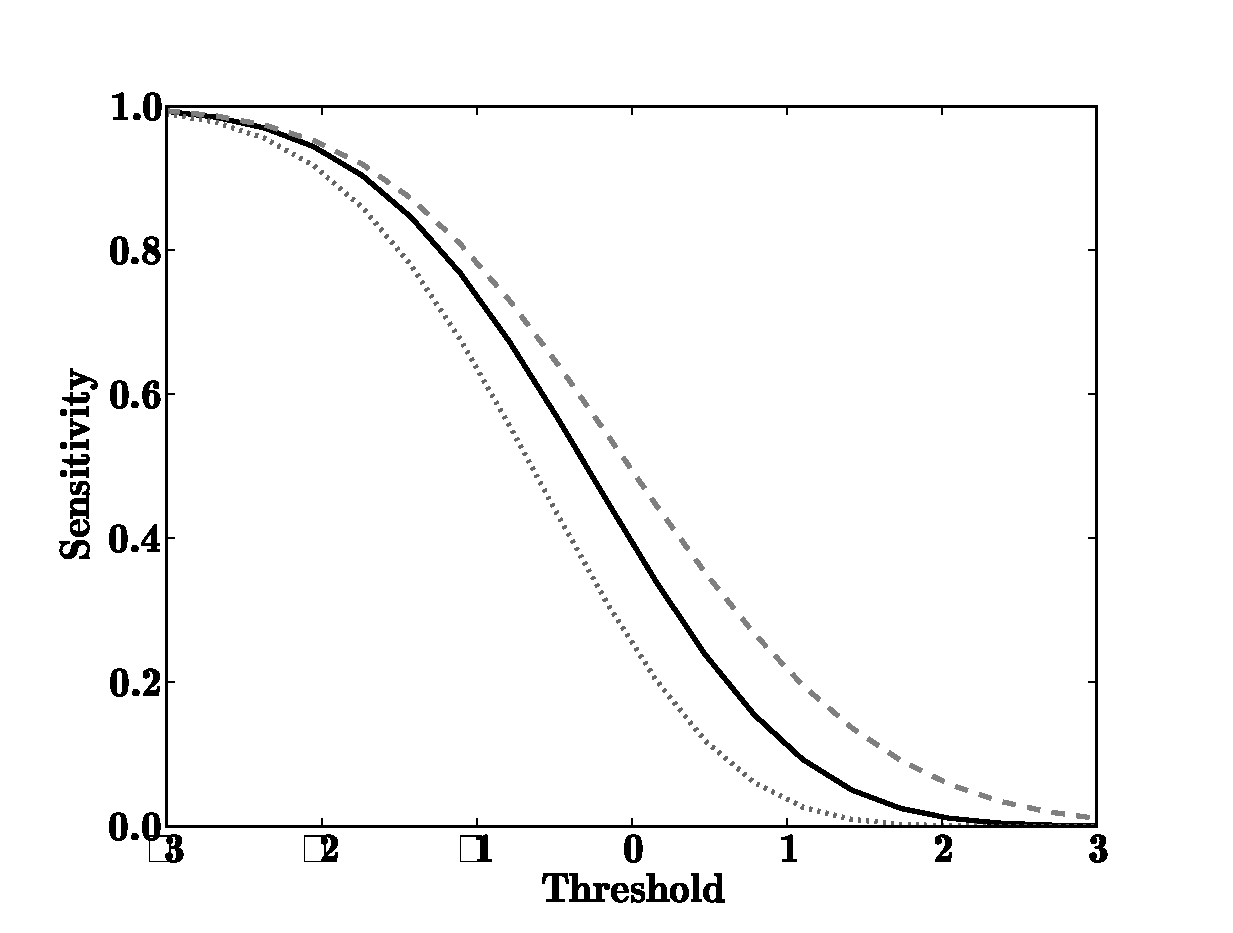
\includegraphics[width=.49\textwidth]{figs/sens_comparison_leafs}}
\subfigure[][]{\label{fig:1b}\includegraphics[width=.3\textwidth]{figs/amazon_pred_varying_mu}}
\subfigure[][]{\label{fig:clinical_roc}\includegraphics[width=0.3\textwidth]{figs/ROC_comparison_leafs}}
\caption{ROC curves for out-of-sample ICD-9 code prediction from patient free-text discharge records 
(\subref{fig:1a},\subref{fig:clinical_roc}). ROC curve for out-of-sample Amazon product category predictions from 
product free-text descriptions \subref{fig:1b}. Figures \subref{fig:1a} and \subref{fig:1b} are a function 
of the prior means of the regression parameters. Figure \subref{fig:clinical_roc} is a function of auxiliary variable threshold. In all figures, solid is 
HSLDA, dashed are independent regressors + sLDA (hierarchical 
constraints on labels ignored), and dotted is HSLDA fit by running LDA first then running 
tree-conditional regressions.}
\label{fig:main_results}
\end{center}
\end{figure}


The results in Figures~\ref{fig:1a} and \ref{fig:1b} suggest that in most cases
it is better to do full joint estimation of HSLDA.  An alternative
interpretation of the same results is that, if one is more sensitive to the
performance gains that result from exploiting the structure of the labels, then
one can, in an engineering sense, get nearly as much gain in label prediction
performance by first fitting LDA and then fitting a hierarchical probit
regression.  There are applied settings in which this could be advantageous.


%\subsection{}
\section{Introduction}
%\section{Related Work}

\label{sec:introduction} 
There exist many sources of unstructured data that have been partially or
completely categorized by human editors.  In this paper we focus on
unstructured text data that has been, at least in part, manually
categorized.  Examples include but are not limited to webpages and curated
hierarchical directories of the same \citep{DMOZ}, product descriptions and
catalogs, %(e.g.~\citep{AMAZON} as available from \citep{SNAP})
and patient records %hospital treatment transcripts
and diagnosis codes assigned to them for bookkeeping and insurance purposes
(e.g.~hospital discharge summaries with 
International Classification of Disease 9th Revision, Clinical Modification
(ICD-9-CM) codes assigned \cite{ICD9}).  In this work we show how to combine
these two sources of information using a single model that allows one to
categorize new text documents automatically, suggest labels that might be
inaccurate, compute improved similarities between documents for information
retrieval purposes, and more. The models and techniques that we develop in
this paper are applicable in other data as well, namely, any unstructured
representations of data that have been hierarchically classified (e.g.,~image
catalogs with bag-of-feature image representations).

There are several challenges entailed in incorporating a hierarchy of labels
into the model. Given a large set of potential labels (often thousands), each
instance has only a small number of labels associated to it. There are no
naturally occurring negative labeling in the data, and the absence of a label
cannot always be interpreted as a negative labeling. 

Our work operates within the framework of topic modeling. Our approach learns
topic models of the underlying data and labeling strategies in a joint model,
while leveraging the hierarchical structure of the labels. For the sake of
simplicity, we focus on is-a hierarchies, but the model can be
applied to other hierarchies. We extend supervised latent Dirichlet
allocation (sLDA)~\cite{BleiMcAuliffe2008} to take advantage of hierarchical
supervision. We propose an efficient way to incorporate hierarchical
information into the model. We hypothesize that the context of labels within
the hierarchy provides valuable information about labeling. 

We demonstrate our model on large, real-world datasets in the clinical and web
retail domains. We observe that hierarchical information is valuable when
incorporated into the learning and improves our primary goal of multi-label
classification. Our results show that a joint, hierarchical model outperforms a
classification with unstructured labels as well as a disjoint model, where the
topic modeling and the hierarchical classification are carried out
independently of each other. 

The remainder of this paper is as follows. Section~\ref{sec:model}
introduces hierarchically supervised LDA (HSLDA), while
Section~\ref{sec:inference} details a sampling approach to inference in HSLDA. 
Section~\ref{sec:related_work} reviews related work, and
Section~\ref{sec:experiments} shows results from applying HSLDA to health care
and web retail data.  

%In this paper we describe the use of a topic model based on supervised
%latent Dirichlet allocation (sLDA) to identify topics within narrative
%discharge summaries and to automate the assignment of diagnostic codes,
%specifically International Classification of Disease 9th Revision,
%Clinical Modification (ICD-9-CM) codes. There are a number of advantages
%to this approach. First, manually coding diagnoses is a time-consuming
%and notoriously unreliable process. Many diagnoses are omitted in
%the final record, and a high error rate is found even in the principal
%diagnoses \citep{Surjan1999}.

%Our main contribution is to show how to utilize supervision in the form of
%hierarchical and (often) multiple labelings in a similar manner. Consider web
%retail data. Web retailers often have both a browse-able product hierarchy and
%free-text descriptions for all products they sell. The situation of each
%product in a product hierarchy (often multiply situated) constitutes a
%multiple, hierarchical labeling of the free-text product descriptions. We
%hypothesize that such hierarchical labels should, at least in theory, provide
%better supervision than the simpler unstructured labels previously considered.
%Results from applying our model to both medical record and web retail data
%suggests that this is likely the case. In particular, we observe gains in our
%primary goal of out-of-sample label prediction that result specifically from
%leveraging hierarchical supervision. 

%\begin{itemize}
%\item Benefits of combining human categorization information into ``topic models''
%\item LDA solved free text
%\item supervised LDA improves LDA (extra info) and allows new inference (predict links, etc.)
%\item amazon, freshdirect, netflix, dmoz, pandora (music genome)
%\end{itemize}


% Informatics journal paper
%
% Despite the growing emphasis on meaningful
%use of technology in medicine, many aspects of medical record-keeping
%remain a manual process. Diagnostic coding for billing and insurance
%purposes is often handled by professional medical coders who must
%explore a patient's extensive clinical record before assigning the
%proper codes. So while electronic health records (EHRs) should be
%adopted by most medical institutions within the next several years,
%largely due to the provisions of HITECH under the American Recovery
%and Reinvestment Act \citep{Blumenthal2009}, there has been little
%movement forward in automating medical coding.

%An automated process would ideally produce a more complete and accurate
%diagnosis lists. Also, this model will reveal information about the
%medical records themselves. For example, we may gain an understanding
%of what a specific code actually means in terms of clinical narratives.
%Similarly, viewing the distribution of topics over discharge summaries
%may reveal information about the latent structure of clinician documentation.
%Lastly, the sLDA model would provide a novel approach to dealing with
%the problem of high dimensionality when representing narrative text
%in a vector space specifically by reducing dimensions from an entire
%vocabulary of potentially tens of thousands of words to a set of several
%dozen topics.

%In this work we extend supervised latent Dirichlet allocation (sLDA)
%\cite{BleiMcAuliffe2008} to take advantage of hierarchical supervision.  sLDA
%is latent Dirichlet allocation (LDA) \cite{Blei2003} augmented with per
%document ``supervision'';  often taking the form of a single numerical or
%categorical ``label.''  More generally this supervision is just extra per
%document data;  for instance its quality or relevance (e.g.~online review
%scores), marks given to written work (e.g.~essay grades), or the number of
%times a web page is linked.  These labels are usually generatively modeled as
%having been conditionally drawn from some distribution that depends on the
%document-specific topic mixture.  It has been demonstrated that the signal
%provided by such supervision can result in better, task-specific document
%models and can also lead to good label prediction for out-of-sample data
%\cite{BleiMcAuliffe2008}. 




\section{Hierarchical Supervised Latent Dirichlet Allocation}
\label{sec:HSLDA}
% !TEX root =  ../../Krantz_style.tex

\label{sec:model} 
%We define here a hierarchically supervised LDA
%model. Although we will focus on document modeling in our description
%and experiments, this model applies equally well to other collections
%of discrete data with hierarchically constrained labels. 

This model (HSLDA) is designed to fit hierarchically, multiply-labeled, bag-of-word data.  We
call groups of bag-of-words data documents (unordered words in text documents, bag of visual feature representations of images, etc.).  Let $w_{n,d}
\in \Sigma$ be the $n$th observation in the $d$th document.  Let $\mathbf{w}_d
= \{w_{1,d},\ldots,w_{1,N_d}\}$ be the  set of $N_d$ observations in document
$d$.  Let there be $D$ such documents and let the size of the vocabulary be
$V=|\Sigma|$.  

Let the set of labels be $\mathcal{L}=\left\{
  l_{1},l_{2},\ldots,l_{\left|\mathcal{L}\right|}\right\} $.  A label in HSLDA corresponds to a node in the graphical model in Figure~\ref{fig:graphical_model}.  A label can either be observed or unobserved.  Documents can be multiply labeled, meaning that subsets of label nodes in the graphical model in Fig.~\ref{fig:graphical_model} can have observed values.  Each label
$l \in \mathcal{L}$, except the root, has a parent $\mathrm{pa}(l) \in \mathcal{L}$
also in the set of labels. 
 We will for exposition purposes assume that this label set has hard ``is-a''
 parent-child constraints (explained later), although this assumption can be
 relaxed at the cost of more computationally complex inference.  Such a label hierarchy forms a multiply rooted tree.   Confused readers may wish to consult Figure \ref{fig:diagnosis_tree} or Figure \ref{fig:product_tree} each of which is a  label-tree graphical model.  
 
 In a label forest a node may be observed (the label was ``applied'' and, for instance, was observed to have value 1), unobserved and unknown, or unobserved and constrained to be either -1 or 1 by the structure of the label space.   Without loss of generality we will consider a tree with a single root $r\in\mathcal{L}$.  Each document has a variable $y_{l,d} \in \{-1,1\}$ for every label which indicates whether the label applies to document $d$ or not.   In most cases $y_{l,d}$ will be unobserved, in some cases we will be able to fix its value because of  constraints on the label hierarchy, and in the relatively minor remainder its value will be observed.  In the applications we demonstrate, only positive labels are observed.   This may not be true of all applications; however, positive-only label imbalance is a common problem.  How we solve this problem will be discussed later.
 
The constraints imposed by an is-a label hierarchy are that if the $l$th label is applied to document $d$, i.e.,~$y_{l,d} = 1$, then all labels in the label hierarchy up to the root are also applied to document $d$, i.e.,~$y_{\mathrm{pa}(l),d} = 1, y_{\mathrm{pa}(\mathrm{pa}(l)),d} = 1, \ldots, y_{r,d}=1.$  Conversely, if a label $l'$ is marked as not applying to a document (i.e.~$y_{l',d}=-1$) then no descendant label of that label can take value 1.   We assume that at least one label is applied to every document.  This is illustrated in Figure~\ref{fig:graphical_model} where the root label is always applied but only some of the descendant labelings are observed as having been applied (diagonal hashing indicates that potentially some of the plated variables are observed).
%To reiterate, these is-a label hierarchy constraints can be relaxed.
%To capture this hierarchical structure we model the labeling of documents
%using a generative cascade of conditional probit regression models.

% generalize to arbitrary codes (not just ICD-9's
%
\begin{figure}[t]
%tbp] %  figure placement: here, top, bottom, or page
 \centering \includegraphics[scale=0.4]{Chapters/chapter1/Graphical_Model-final} \caption{Hierarchically supervised latent Dirichlet allocation (HSLDA) graphical model.}


\label{fig:graphical_model} 
\end{figure}

In HSLDA, the bag-of-word document data is modeled using LDA with
 full, hierarchical topic estimation (i.e. with the global topic estimated too rather than assumed).
%In HSLDA, documents are modeled using the LDA mixed-membership mixture model
%with global topic estimation. 
Label responses are modeled using a conditional
hierarchy of probit regressors and will be discussed next. The full HSLDA graphical model is given in
Figure~\ref{fig:graphical_model}.

 

\subsection{Generative Model}

In the following box  the HSLDA generative model  is given for the ``is-a hierarchy'' set of label constraints.   In the box and what follows in this chapter, $K$ is the number of LDA
``topics'' (distributions over the elements of $\Sigma$), $\boldsymbol\phi_k$
is a distribution over ``words,'' $\boldsymbol\theta_d$ is a document-specific
distribution over topics, $\boldsymbol\beta$ is a global distribution over
topics, Dir$_{K}(\cdot)$ is a $K$-dimensional Dirichlet distribution,
$\mathcal{N}_{K}(\cdot)$ is the $K$-dimensional Normal distribution,
$\mathbf{I}_{K}$ is the $K$ dimensional identity matrix,  $\mathbf{1}_d$ is the
$d$-dimensional vector of all ones, and $\mathbb{I}(\cdot)$ is an indicator
function that takes the value $1$ if its argument is true and $0$ otherwise.

 %as well as the mean, $\boldsymbol\mu$, and the standard deviation, $\sigma$,
%used in a normal prior distribution. The hyper-parameters $\alpha^{\prime}$,
%$\alpha$, and $\gamma$ are weight parameters for Dirichlet prior
%distributions. 


%We will now describe the stochastic generative process which defines
%our model. The 
%Given the number of topics, K, and broad gamma priors on hyperparameters,
%the generative process is as follows: 
\begin{shortbox}
\Boxhead{HSLDA Generative Model}
\begin{enumerate}
\item For each topic $k=1,\ldots,K$

\begin{itemize}
\item Draw a distribution over words $\boldsymbol\phi_{k}\sim{\rm Dir}_{V}(\gamma\mathbf{1}_V)$%,
%where $\mathbf{1}$ is a vector of ones of length $V$ 
\end{itemize}
\item For each label $l\in\mathcal{L}$

\begin{itemize}
\item Draw a label weight vector $\boldsymbol\eta_{l}\mid\mu,\sigma\sim\mathcal{N}_{K}(\mu \mathbf{1}_K,\sigma \mathbf{I}_{K})$  
\end{itemize}
\item Draw the global topic proportions $\boldsymbol\beta\mid\alpha'\sim{\rm Dir}_{K}\left(\alpha^{\prime}\mathbf{1}_K\right)$
\item For each document $d=1,\ldots,D$

\begin{itemize}
\item Draw topic proportions $\boldsymbol\theta_d\mid\boldsymbol\beta,\alpha\sim{\rm Dir}_{K}\left(\alpha\boldsymbol\beta\right)$ 
\item For $n=1,\ldots,N_{d}$

\begin{itemize}
\item Draw topic assignment $z_{n,d}\mid\boldsymbol\theta_d\sim{\rm Multinomial}(\boldsymbol\theta_d)$ 
\item Draw word $w_{n,d}\mid z_{n,d},\boldsymbol\phi_{1:K}\sim{\rm Multinomial}(\boldsymbol\phi_{z_{n,d}})$ 
\end{itemize}
\item Set $y_{r,d} = 1$
\item For each label $l$ in a breadth first traversal of $\mathcal{L}$ starting at the children of  root $r$

\begin{itemize}
\item Draw 
\begin{eqnarray}\lefteqn{a_{l,d}\mid \bar{\mathbf{z}}_d,\boldsymbol\eta_{l},y_{\mathrm{pa}(l),d}}\nonumber \\&\sim&\begin{cases}
\mathcal{N}(\bar{\mathbf{z}}^{T}_d\boldsymbol\eta_{l},1), & y_{\mathrm{pa}(l),d}=1 \\
\mathcal{N}(\bar{\mathbf{z}}^{T}_d\boldsymbol\eta_{l},1)\mathbb{I}(a_{l,d}<0), & y_{\mathrm{pa}(l),d}=-1 \end{cases}\label{zero_0}\end{eqnarray} %\item Draw $a_{l, d} \ | \ z_{1:N_d,d}, \boldsymbol\beta_l \sim \mathcal{N} \left(\bar z_d^{T} \boldsymbol\beta_{l},1\right)$, where $\bar z_d=N_d^{-1}\sum_{n=1}^{N_d}z_{n,d}$ 
 
\item Apply label $l$ to document $d$ according to $a_{l,d}$ \begin{eqnarray}\hspace{-2.2cm}
y_{l,d}\mid a_{l,d}=\begin{cases}
\;\;\, 1 & \text{if \ensuremath{a_{l,d}>0}}  \\% and \ensuremath{y_{{\rm \mathrm{pa}}(l),d}=1}}\\
 -1 & \text{otherwise} \end{cases}\label{zero_1}\end{eqnarray}
 
\end{itemize}
\end{itemize}
\end{enumerate}
\label{box:generative_model}
\end{shortbox}

Here $\bar{\mathbf{z}}_d^T = [\bar{z}_{1}, \ldots, \bar{z}_k, \ldots, \bar{z}_K]$ is the empirical topic distribution for document $d$, in which each entry is the percentage of the words in that document that come from topic $k$, $\bar{z}_{k}=N_{d}^{-1}\sum_{n=1}^{N_d}\mathbb{I}(z_{n,d}=k).$  

The second half of step 4 is what is referred to as supervision in the supervised LDA literature.  This is where the hierarchical classification of the bag-of-words data takes place and the is-a label constraints are enforced.  For every label $l \in \mathcal{L}$, both the empirical topic distribution for document $d$ and whether or not its parent label was applied (i.e.~$\mathbb{I}(y_{\mathrm{pa}(l),d}=1)$) are used to determine whether or not  label $l$ is to be applied to  document $d$ as well.    \eqref{zero_0} and \eqref{zero_1} comprise a probit regression model in an auxiliary variable formulation (see Section \ref{sec:probit_review}).   Note that in the case that the parent label is applied, i.e.~$y_{\mathrm{pa}(l),d}=1,$ the child label $y_{l,d}$ is applied with probability $P(\bar{\mathbf{z}}^{T}_d\boldsymbol\eta_{l}>0).$  This is a conditional probit regression model for classification where $\boldsymbol\eta_l$ are the class-conditional regression parameters.  The auxiliary variables $a_{l,d}$ make inference tractable but are not fundamental to the model -- only the labels and regression parameters are actually of interest.

Note that $y_{l,d}$ can only be applied to document $d$  (set to 1) if its parent label $\mathrm{pa}(l)$ was also applied (these expressions are specific to is-a constraints but could be modified to accommodate different constraints between labels).  Note that multiple labels can be applied to the same document.  The regression coefficients $\boldsymbol\eta_l$ which generate the labels are independent a priori, however, the hierarchical coupling in this model and conditional label dependency structure induces a posteriori dependence.   The net effect of this conditional hierarchy of profit regressors is that child label predictors deeper in the label hierarchy are able to focus on finding features that distinguish label paths in the tree, conditioned on the fact that all the children of any particular node are by design members of some more general parent set.  It should be clear that one can trivially restrict this hierarchy to a depth one hierarchy recovering SLDA with probit link and univariate categorical labels.  Also, one can nearly as easily make the conditional classification at each node multi-class rather than single-class if more than one label at each node is required.  In many cases, however, a binary indicator along with a deeper or more complex tree is sufficient.
%We believe this to be a significant source of the empirical label prediction improvement we observe experimentally.  We test this hypothesis in Section~\ref{sec:experiments}.

Note that the choice of variables $a_{l,d}$ and how they are distributed were  driven at least in part by posterior inference efficiency considerations (see Appendix \ref{sec:probit_review}).  In particular, choosing probit-style auxiliary variable distributions for the $a_{l,d}$'s  yields conditional posterior distributions for both the auxiliary variables \eqref{eqn:a_l_d} and the regression coefficients \eqref{eqn:regression_param_conditional} which are analytic.  This simplifies posterior inference substantially.  A review of probit regression can be found near the end of this chapter in Section \ref{sec:probit_review}.

%Probit regression is similar to logistic regression except that it uses the standard normal distribution cumulative distribution function (CDF) rather than the logistic sigmoid link function.  The inverse of the normal CDF is is known as the probit function.  
%The latent variables $a_{l,d}$ are
%auxiliary variables because the are introduced to make exact Gibbs
%sampling possible and are not of primary interest.

%This type of generative model is known as a probit regression model.
%Probit regression models are a type of discriminative probabilistic
%model similar to logistic regression. However, instead of using the
%logistic sigmoid as the link function, the probit regression model
%uses the CDF for a standard normal distribution - the inverse of which
%is known as the probit. In this case, the regression is conditional
%on the parents according to the constraints of the labeling hierarchy.

\subsection{Dealing with Label Imbalance}

In the common case where no negative labels are observed (like the example applications we consider in Section~\ref{sec:example_applications}), the model must be explicitly biased towards generating  negative labels in order to keep it from learning to only assign positive labels to all documents.   This is a common problem in modeling with unbalanced labels.  To see how this model can achieve this we draw the reader's attention to the $\mu$ parameter and, to a lesser extent, the $\sigma$ parameter above.  Because $\bar{\mathbf{z}}_d$ is always positive, setting $\mu$ to a negative value results in a bias towards negative labelings, i.e.~for large negative values of $\mu$, all labels become a priori more likely to be negative ($y_{l,d}=-1$).  We explore the effect of $\mu$ on out-of-sample label prediction performance in Section~\ref{sec:example_applications}.   In a very real way $\mu$ is a knob that can be adjusted both before inference to induce a broad array of out-of-sample performance characteristics that vary along classical axes like specificity, recall, and accuracy.  A similar but less principled solution can be effected by changing the decision boundary from $0$ in \eqref{zero_0} and \eqref{zero_1}.  This technique can be used to vary out-of-sample label bias after learning.

%we apply an informative
%prior to the regression parameters, $\mathbf{\boldsymbol\beta}_{\mathcal{L}}$,
%in the form of a negative prior that encodes a bias towards being
%truly negative in the absence of a label.




\subsection{Intuition}
\label{sec:intuition}
% !TEX root =  ../../Krantz_style.tex

%This chapter covers one way to utilize supervision in the form of
%hierarchical and (often) multiple labelings in a similar manner. 
To help ground this abstract graphical model, recall the 
retail data example application. We asserted that  retailers often have both a browse-able product hierarchy and
free-text descriptions for all products they sell. The situation of each
product in a product hierarchy (often multiply situated) constitutes a
multiple, hierarchical labeling $\mathbf{y}_d$ of the free-text product descriptions  $\mathbf{w}_d$ for all products $d.$     Note that a single product can be placed in the hierarchy in multiple places.  This corresponds to multiple paths in the label hierarchy having labels that are all applied.  HSLDA assumes that the free-text descriptions of all of the products in a particular node in the product hierarchy must be related.  It also assumes that products deeper in the product hierarchy are  described using language that is similar to that used to describe products in their parent classes.  For instance basketballs are probably described using language that is similar to that used to describe other basketballs, other balls, and more general sporting goods.   In both the lay and technical senses, similar products should have product descriptions that share topics.   If topic proportions are indicative of the text describing products that are grouped together, the key HSLDA assumption is that it should then be possible to use those proportions to decide (via probit classification) whether or not a particular product should be situated at a particular node in the product hierarchy.  Conversely, that certain groups of products are known to be clustered together should inform the kinds of topics that are inferred from the product descriptions.



%hierarchical labels should, at least in theory, provide
%better supervision than the simpler unstructured labels previously considered.
%Results from applying our model to both medical record and web retail data
%suggests that this is likely the case. In particular, we observe gains in our
%primary goal of out-of-sample label prediction that result specifically from
%leveraging hierarchical supervision. 


%
%We extend supervised latent Dirichlet
%allocation (sLDA)~\cite{BleiMcAuliffe2008} to take advantage of hierarchical
%supervision. We propose an efficient way to incorporate hierarchical
%information into the model. We hypothesize that the context of labels within
%the hierarchy provides valuable information about labeling. 
%


%The remainder of this chapter is arranged as follows. Section~\ref{sec:model}
%introduces hierarchically supervised LDA (HSLDA), while
%Section~\ref{sec:inference} details a sampling approach to inference in HSLDA. 
%and
%Section~\ref{sec:experiments} shows results from applying HSLDA to health care
%and web retail data.  

%In this paper we describe the use of a topic model based on supervised
%latent Dirichlet allocation (sLDA) to identify topics within narrative
%discharge summaries and to automate the assignment of diagnostic codes,
%specifically International Classification of Disease 9th Revision,
%Clinical Modification (ICD-9-CM) codes. There are a number of advantages
%to this approach. First, manually coding diagnoses is a time-consuming
%and notoriously unreliable process. Many diagnoses are omitted in
%the final record, and a high error rate is found even in the principal
%diagnoses \cite{Surjan1999}.

%Our main contribution is to show how to utilize supervision in the form of
%hierarchical and (often) multiple labelings in a similar manner. Consider web
%retail data. Web retailers often have both a browse-able product hierarchy and
%free-text descriptions for all products they sell. The situation of each
%product in a product hierarchy (often multiply situated) constitutes a
%multiple, hierarchical labeling of the free-text product descriptions. We
%hypothesize that such hierarchical labels should, at least in theory, provide
%better supervision than the simpler unstructured labels previously considered.
%Results from applying our model to both medical record and web retail data
%suggests that this is likely the case. In particular, we observe gains in our
%primary goal of out-of-sample label prediction that result specifically from
%leveraging hierarchical supervision. 

%\begin{itemize}
%\item Benefits of combining human categorization information into ``topic models''
%\item LDA solved free text
%\item supervised LDA improves LDA (extra info) and allows new inference (predict links, etc.)
%\item amazon, freshdirect, netflix, dmoz, pandora (music genome)
%\end{itemize}


% Informatics journal paper
%
% Despite the growing emphasis on meaningful
%use of technology in medicine, many aspects of medical record-keeping
%remain a manual process. Diagnostic coding for billing and insurance
%purposes is often handled by professional medical coders who must
%explore a patient's extensive clinical record before assigning the
%proper codes. So while electronic health records (EHRs) should be
%adopted by most medical institutions within the next several years,
%largely due to the provisions of HITECH under the American Recovery
%and Reinvestment Act \cite{Blumenthal2009}, there has been little
%movement forward in automating medical coding.

%An automated process would ideally produce a more complete and accurate
%diagnosis lists. Also, this model will reveal information about the
%medical records themselves. For example, we may gain an understanding
%of what a specific code actually means in terms of clinical narratives.
%Similarly, viewing the distribution of topics over discharge summaries
%may reveal information about the latent structure of clinician documentation.
%Lastly, the sLDA model would provide a novel approach to dealing with
%the problem of high dimensionality when representing narrative text
%in a vector space specifically by reducing dimensions from an entire
%vocabulary of potentially tens of thousands of words to a set of several
%dozen topics.

%In this work we extend supervised latent Dirichlet allocation (sLDA)
%\cite{BleiMcAuliffe2008} to take advantage of hierarchical supervision.  sLDA
%is latent Dirichlet allocation (LDA) \cite{Blei2003} augmented with per
%document ``supervision'';  often taking the form of a single numerical or
%categorical ``label.''  More generally this supervision is just extra per
%document data;  for instance its quality or relevance (e.g.~online review
%scores), marks given to written work (e.g.~essay grades), or the number of
%times a web page is linked.  These labels are usually generatively modeled as
%having been conditionally drawn from some distribution that depends on the
%document-specific topic mixture.  It has been demonstrated that the signal
%provided by such supervision can result in better, task-specific document
%models and can also lead to good label prediction for out-of-sample data
%\cite{BleiMcAuliffe2008}. 




\section{Inference}
\label{sec:inference}

\label{sec:inference}
Our inference goal  is to obtain a representation of the posterior distribution
of the latent variables in the model.  The posterior distribution we seek does not have a simple analytic form from which exact samples can be drawn.
This is usually the case for posterior distributions of non-trivial
probabilistic models and suggests a approximating the posterior distribution by sampling.

In this section we derive the conditional distributions required to sample from the HSLDA posterior distribution using Markov chain Monte Carlo. 

XXX  A very brief review of Markov chain Monte Carlo can be found in Section \ref{sec:mcmc} at the end of this chapter.  XXX

The HSLDA sampler, like the collapsed Gibbs samplers for LDA \cite{Griffiths04}, is itself a collapsed Gibbs sampler in which all of the latent variables that can be analytically marginalized are.  Among others, the parameters $\boldsymbol{\phi}_{1:K}$
and $\boldsymbol{\theta}_{1:D}$ are analytically marginalized prior to deriving the following conditional distributions for sampling.  
  It will often be the
case that the set of labels $\mathcal{L}$ is not fully observed for
every document. We will define $\mathcal{L}_{d}$ to be the subset
of labels which have been observed for document $d$. In an is-a hierarchical regression  it is straightforward
to marginalize the variables $a_{l^{\prime},d}$ and $y_{l^{\prime},d}$
for $l^{\prime}\in\mathcal{L}\backslash\mathcal{L}_{d}$ simply by ignoring them. 
%We can also integrate out the parameters $\boldsymbol{\phi}_{1:K}$
%and $\boldsymbol{\theta}_{1:D}$ as in \cite{Griffiths04}.
 The remaining latent variables (those that are not collapsed out) are $\mathbf{z}=\{z_{1:N_{d},d}\}_{d=1,\ldots,D},\boldsymbol\eta=\{\boldsymbol\eta_{l}\}_{l\in\mathcal{L}},\mathbf{a}=\{a_{l^{\prime},d}\}_{l^{\prime}\in\mathcal{L}_{d},d=1,\ldots,D},\boldsymbol\beta,\alpha,\alpha^{\prime}$
and $\gamma$.


%We will appeal to one of the common methods
%for approximating posterior distributions in the face of intractable
%normalization factors: Markov chain Monte Carlo (MCMC) sampling. 
%Since
% the conditional distributions
%for all variables are relatively simple (enumeration and, in the case of the profit regression coefficients, conjugate) we will use Gibbs sampling. %In particular, we will derive a collapsed Gibbs sampler.
%Given an observation of a set of observed labels and a document, the posterior distribution for the latent variables is
%\begin{equation}
%p\left(\theta,z_{1:N},\phi_{1:K},\boldsymbol\eta_{i_{l,c}\in\mathcal{I}},a_{i_{l,c}\in\mathcal{I}},\boldsymbol\beta,\alpha,\alpha',\gamma\mid w_{1:N},y_{i_{l,c}\in\mathcal{I}};\sigma,\lambda\right)\label{eq:Posterior}\end{equation}
%\[
%=\frac{p\left(\theta,z_{1:N},\phi_{1:K},\boldsymbol\eta_{i_{l,c}\in\mathcal{I}},a_{i_{l,c}\in\mathcal{I}},\boldsymbol\beta,\alpha,\alpha',\gamma,w_{1:N},y_{i_{l,c}\in\mathcal{I}};\sigma,\lambda\right)}{\int_{\theta,\phi,a,\boldsymbol\eta,\alpha,\alpha',\boldsymbol\beta,\gamma}\sum_{z}p\left(\theta,z_{1:N},\phi_{1:K},\boldsymbol\eta_{i_{l,c}\in\mathcal{I}},a_{i_{l,c}\in\mathcal{I}},\boldsymbol\beta,\alpha,\alpha',\gamma,w_{1:N},y_{i_{l,c}\in\mathcal{I}};\sigma,\lambda\right)}\]
%
%

\subsection{Gibbs Sampler}
 Let $\mathbf{a}$ be the set of all auxiliary variables, $\mathbf{w}$  the set of all words, $\boldsymbol\eta$  the set of all regression coefficients, and  $\mathbf{z}\backslash z_{n,d}$  the set $\mathbf{z}$ with element $z_{n,d}$ removed.  %The conditional posterior distribution of the latent topic indicators is
 %We use the notation $\mathbf{z}_{-(n,d)}$ to
%denote $\mathbf{z}_d\backslash z_{n,d}$. %, marginalizing
%$\theta_{1:D}$ and $\phi_{1:K}$. For details regarding collapsing
%in LDA models see \cite{Griffiths04}. 



%\subsection{Sampling latent topic indicators}
%$p(z_{n,d}\mid\mathbf{z}_{-(n,d)},\mathbf{a},\mathbf{w},\mathbf{\boldsymbol\eta},\alpha,\boldsymbol\beta,\gamma)$}

First we consider the conditional distribution of $z_{n,d}$ (the assignment variable
for each word $n=1,\ldots,N_{d}$ in documents $d=1,\ldots,D$). 
%The
%conditional distribution does not include $\theta_{1:D}$ and $\phi_{1:K}$
%because they have been integrated out as in the collapsed Gibbs sampler
%\cite{Griffiths04}. 
%The conditional distribution of $z_{n,d}$ is
%proportional to the joint distribution of its markov blanket. \begin{equation}
%p\left(z_{d,n}\mid\mathbf{z_{-\left(d,n\right)}},\mathbf{a},\mathbf{w},\mathbf{\boldsymbol\eta},\alpha,\boldsymbol\beta,\gamma\right)\propto p\left(z_{d,n},\mathbf{z_{-\left(d,n\right)}},\mathbf{a},\mathbf{w},\mathbf{\boldsymbol\eta},\alpha,\boldsymbol\beta,\gamma\right)\end{equation}
Following the factorization of the model (refer again to Figure~\ref{fig:graphical_model}), we can write
\begin{eqnarray*}
\lefteqn{p\left(z_{n,d}\mid\mathbf{z}_d\backslash z_{n,d},\mathbf{a},\mathbf{w},\mathbf{\boldsymbol\eta},\alpha,\boldsymbol\beta,\gamma\right)}\\
&\propto&\prod_{l\in\mathcal{L}_{d}}p\left(a_{l,d}\mid\mathbf{z},\boldsymbol\eta_{l}\right)p\left(z_{n,d}\ |\ \mathbf{z}_d\backslash z_{n,d},\mathbf{a},\mathbf{w},\alpha,\boldsymbol\beta,\gamma\right).\end{eqnarray*}
 The product is only over the subset of labels $\mathcal{L}_{d}$
which have been observed for document $d$. By isolating terms that
depend on $z_{n,d}$ and absorbing all other terms into a normalizing
constant as in \cite{Griffiths04} we find 
\begin{eqnarray}
\lefteqn{p\left(z_{n,d}=k\mid\mathbf{z}\backslash z_{n,d},\mathbf{a},\mathbf{w},\mathbf{\boldsymbol\eta},\alpha,\boldsymbol\beta,\gamma\right)\propto} \label{eq:z-likelihood} \\
 & \hspace{2cm}\left(c_{\left(\cdot\right),d}^{k,-\left(n,d\right)}+\alpha\boldsymbol\beta_{k}\right)\frac{c_{w_{n,d},\left(\cdot\right)}^{k,-\left(n,d\right)}+\gamma}{\left(c_{\left(\cdot\right),\left(\cdot\right)}^{k,-\left(n,d\right)}+V\gamma\right)}\prod_{l\in\mathcal{L}_{d}}\exp\left\{ -\frac{\left(\bar{\mathbf{z}}_{d}^{T}\boldsymbol\eta_{l}-a_{l,d}\right)^{2}}{2}\right\}\nonumber\end{eqnarray}
 where $c_{v,d}^{k,-\left(n,d\right)}$ is the number
of words of type $v$ in document $d$ assigned to topic $k$ omitting
the $n$th word of document $d$. The subscript $(\cdot)$'s
indicate to sum over the range of the replaced variable, i.e.~$ {c_{w_{n,d},\left(\cdot\right)}^{k,-\left(n,d\right)}} = \sum_d {c_{w_{n,d},d}^{k,-\left(n,d\right)}}$.  Here $\mathcal{L}_{d}$ is the set of labels which are observed for document $d$.  We sample from \eqref{eq:z-likelihood}  by enumeration and implicit normalization.
%
%Given Equation \ref{eq:z-likelihood}, $p\left(z_{d,n}\mid\mathbf{z}_{-\left(d,n\right)},\mathbf{a},\mathbf{w},\mathbf{\boldsymbol\eta},\alpha,\boldsymbol\beta,\gamma\right)$
%can be sampled through enumeration. 

The conditional posterior distribution of the regression coefficients is given by 
\begin{equation}
p(\boldsymbol\eta_{l}\mid\mathbf{z},\mathbf{a},\sigma) = \mathcal{N}(\hat{\boldsymbol\mu}_{l},\hat{\mathbf{\Sigma}})\label{eqn:regression_param_conditional}
\end{equation}
$\boldsymbol\eta_{l}$ for $l\in\mathcal{L}$. Given that $\boldsymbol\eta_{l}$
and $a_{l,d}$ are distributed normally, the posterior distribution
of $\boldsymbol\eta_{l}$ is normally distributed with mean $\hat{\boldsymbol\mu}_{l}$
and covariance $\hat{\mathbf{\Sigma}}.$% such that % (probably not the right place for this) We evaluated the model over various values of $\sigma$ where $\sigma=\left\{ 0.01,0.1,0.25,1,2\right\} $.
where
\begin{equation*}
\hat{\boldsymbol\mu}_{l}  =  \hat{\mathbf{\Sigma}}\left(\mathbf{1}\frac{\mu}{\sigma}+\bar{\mathbf{Z}}^{T}\mathbf{a}_{l}\right) \qquad \hat{\mathbf{\Sigma}}^{-1}  =  \mathbf{I}\sigma^{-1}+\bar{\mathbf{Z}}^{T}\bar{\mathbf{Z}}
.\end{equation*}
Here $\bar{\mathbf{Z}}$ is a $D\times K$ matrix
such that row $d$ of $\mathbf{\bar{Z}}$ is $\bar{\mathbf{z}}_{d}$, and $\mathbf{a}_{l}=[a_{l,1},a_{l,2},\ldots,a_{l,D}]^{T}$.  The simplicity of this conditional distribution follows from the choice of probit regression  \cite{Albert_Chib_1993}; the specific form of the update is a standard result from Bayesian normal  linear regression \cite{gelmanbda04}. 
%p\left(\boldsymbol\eta_{i_{l,c}}\mid\mathbf{z}_{1:D},\mathbf{a};\sigma\right)=\mathcal{N}\left(\boldsymbol\eta_{i_{l,c}}\mid\hat{\mu}_{i},\hat{\Sigma}_{i}\right)\end{equation}
%\[
%\[
%\subsection{$p\left(a_{l,d}\mid\mathbf{z},\mathbf{Y},\mathbf{\boldsymbol\eta}\right)$}
%and \textmd{$p\left(y_{m,i}\mid\mathbf{a}\right)$}}
%The auxiliary variables $a_{l,d}$ must be sampled for documents $d=1,\ldots,D$
%and $l\in\mathcal{L}_{d}$. The conditional posterior distribution
%of 
It also is a standard probit regression result that the conditional posterior
distribution of $a_{l,d}$ is a truncated normal
distribution~\cite{Albert_Chib_1993}. 
\begin{eqnarray*}
\lefteqn{p\left(a_{l,d}\mid\mathbf{z},\mathbf{Y},\mathbf{\boldsymbol\eta}\right)}\\&\propto&
\begin{cases}
\exp\left\{ -\frac{1}{2}\left(a_{l,d}-\boldsymbol\eta_{l}^{T}\mathbf{\bar{z}}_{d}\right)\right\} \mathbb{I}\left(a_{l,d}y_{l,d}>0\right)\mathbb{I}(a_{l,d}<0) , & y_{\mathrm{pa}(l),d}=-1\\
\exp\left\{ -\frac{1}{2}\left(a_{l,d}-\boldsymbol\eta_{l}^{T}\mathbf{\bar{z}}_{d}\right)\right\} \mathbb{I}\left(a_{l,d}y_{l,d}>0\right) , & y_{\mathrm{pa}(l),d}=1\end{cases}\label{eqn:a_l_d}\end{eqnarray*}

%\begin{equation}
%p\left(a_{l,d,}\mid\mathbf{z},\mathbf{Y},\mathbf{\boldsymbol\eta}\right)\propto\frac{1}{\sqrt{2\pi}}\exp\left\{ -\frac{1}{2}\left(a_{l,d}-\boldsymbol\eta_{l}^{T}\mathbf{\bar{z}}_{d}\right)\right\} \mathbb{I}\left(a_{l,d}y_{l,d}>0\right).\label{eqn:a_l_d}\end{equation}
% This conditional distribution can be sampled using an inverse CDF
%method. %However, if $y_{d,i_{l,c}}$ is unobserved then $a_{d,i_{l,c}}$must
%be sampled jointly with $y_{d,i_{l,c}}$ to ensure that the Markov
%chain is ergodic. Suppose that $a_{d,i_{l,c}}$ is sampled to have
%a negative value and $y_{d,i_{l,c}}$ is apporopriately sampled at
%-1. Although there exist valid states where $a_{d,i_{l,c}}>0$ and
%$y_{d,i_{l,c}}=1$, they will never be reached by such a Markov chain
%since $p\left(a_{d,i_{l,c}}<0\mid y_{d,i_{l,c}}=-1\right)=1$ and
%$p\left(y_{d,i_{l,c}}=-1\mid a_{d,i_{l,c}}<0\right)=1$. Therefore,
%to ensure ergodicity, $a_{d,i_{l,c}}$and $y_{d,i_{l,c}}$ must be
%sampled from the joint distribution as shown in Equation \ref{eq:Probit-Joint}.
%\begin{equation}
%p\left(a_{d,i_{l,c}},y_{d,i_{l,c}}\mid\mathbf{z},\mathbf{Y}_{-\left(d,i_{l,c}\right)},\mathbf{\boldsymbol\eta}\right)\propto p\left(y_{i_{l,c}}\mid\mathbf{a},\mathbf{y}_{-\left(l,c\right)}\right)p\left(a_{d,i_{l,c}}\mid\mathbf{z},\mathbf{Y},\mathbf{\boldsymbol\eta}\right)\end{equation}
%\begin{equation}
%p\left(y_{i_{l,c}}\mid\mathbf{a},\mathbf{y}_{-\left(l,c\right)}\right)=\delta\left(sign\left(a_{d,i_{l,c}}\right)=y_{i_{l,c}}\right)p\left(y_{i_{l,c}}\mid y_{parents_{l,c}}\right)\prod_{i_{\hat{l},\hat{c}}\in children_{l,c}}p\left(y_{i_{\hat{l},\hat{c}}}\mid y_{i_{l,c}}\right)\end{equation}
%\begin{equation}
%p\left(y_{i_{l,c}}=-1\mid y_{parent{}_{l,c}}\right)=\begin{cases}
%1, & y_{parent_{l,c}}=-1\\
%0.5, & y_{parent_{l,c}}=1\end{cases}\end{equation}
%\[
%p\left(a_{d,i_{l,c}},y_{d,i_{l,c}}\mid\mathbf{z},\mathbf{Y}_{-\left(d,i_{l,c}\right)},\mathbf{\boldsymbol\eta}\right)\]
%\begin{equation}
%=\begin{cases}
%\mathcal{N}\left(a_{d,i_{l,c}}\mid\bar{z}^{T}\boldsymbol\eta_{i_{l,c}},1\right)p\left(y_{d,i_{l,c}}\mid a_{d,i_{l,c}}\right), & y_{parent_{l,c}}=1,\forall y_{i_{\hat{l},\hat{c}}}\in y_{children_{l,c}},y_{i_{\hat{l},\hat{c}}}=-1\\
%trunc\mathcal{N}^{-}\left(a_{d,i_{l,c}}\mid\bar{z}^{T}\boldsymbol\eta_{i_{l,c}},1\right)\delta\left(y_{d,i_{l,c}}=-1\right), & y_{parent_{l,c}}=-1\\
%trunc\mathcal{N}^{+}\left(a_{d,i_{l,c}}\mid\bar{z}^{T}\boldsymbol\eta_{i_{l,c}},1\right)\delta\left(y_{d,i_{l,c}}=1\right), & \exists y_{i_{\hat{l},\hat{c}}}\in y_{children_{l,c}}\setminus y_{i_{\hat{l},\hat{c}}}=1\\
%0 & otherwise\end{cases}\end{equation}
%where $\mathbf{Y}_{-\left(d,i_{l,c}\right)}$ denotes all of the response
%variables excluding the response variable being sampled.
%
%
%
%\subsection{$p\left(\boldsymbol\beta\mid\mathbf{z},\alpha^{\prime},\alpha\right)$}

%Note that care must be taken to initialize the Gibbs sampler in a valid state.

HSLDA employs a hierarchical Dirichlet prior over topic assignments (i.e.,~$\boldsymbol\beta$ is estimated from data rather than fixed a priori).  This has been shown to improve the quality and stability of inferred topics \cite{WallachMiMc2009}. 
%This prior
%shares many features with the hierarchical Dirichlet process and inference
%over this distribution proceeds in a very similar fashion.
%
Sampling $\boldsymbol\beta$, the vector of global topic proportions,   can be done using the ``direct assignment''
method of \cite{TehJorBea2006} \begin{equation}
\boldsymbol\beta\mid\mathbf{z},\alpha^{\prime},\alpha\sim{\rm Dir}\left(m_{\left(\cdot\right),1}+\alpha^{\prime},m_{\left(\cdot\right),2}+\alpha^{\prime},\ldots,m_{\left(\cdot\right),K}+\alpha^{\prime}.\right)\end{equation}
Here $m_{d,k}$ are auxiliary variables that are required to sample the posterior distribution of $\boldsymbol\beta$.  Their conditional posterior distribution is sampled according to
 \begin{equation}
p\left(m_{d,k}=m\mid\mathbf{z},\mathbf{m}_{-\left(d,k\right)},\boldsymbol\beta\right)=\frac{\Gamma\left(\alpha\boldsymbol\beta_{k}\right)}{\Gamma\left(\alpha\boldsymbol\beta_{k}+c^k_{(\cdot),d}\right)}s\left(c^k_{(\cdot),d},m\right)\left(\alpha\boldsymbol\beta_{k}\right)^{m}\end{equation}
where $s\left(n,m\right)$ represents stirling numbers of the first
kind.


%\subsection{$p\left(\alpha\right)$, $p\left(\alpha'\right)$, $p\left(\gamma\right)$}

The hyperparameters $\alpha$, $\alpha^{\prime}$, and $\gamma$ are
%given broad ${\rm Gamma}(1,1000)$ prior distributions and 
sampled
using Metropolis-Hastings. 





\section{Example Applications}

\label{sec:example_applications}
% !TEX root =  ../../Krantz_style.tex

%Having described HSLDA and given details on how to do inference in it, we turn to demonstrations of using HSLDA to solve problems from  two different domains: predicting medical
%diagnosis codes from hospital discharge summaries and predicting product
%categories from Amazon.com product descriptions.

%In the section we describe the application of HSLDA for prediction
%in two hierarchically structured domains. Firstly, we describe using
%discharge summaries to predict diagnoses, encoded as ICD-9 codes.
%Discharge summaries are documents that are authored by clinicians
%to summarize the course of a hospitalization. ICD-9 codes are used
%mainly for billing purposes to indicate the conditions for which a
%patient was treated. Secondly, we describe using Amazon.com product
%descriptions to predict product categories.

\subsection{Hospital Discharge Summaries and ICD-9 Codes}

 Despite the growing emphasis on meaningful
use of technology in medicine, many aspects of medical record-keeping
remain a manual process. In the US, diagnostic coding for billing and insurance
purposes is often handled by professional medical coders who must
explore a patient's extensive clinical record before assigning the
proper codes. %So while electronic health records (EHRs) should be
%adopted by most medical institutions within the next several years,
%largely due to the provisions of HITECH under the American Recovery
%and Reinvestment Act \cite{Blumenthal2009}, there has been little
%movement forward in automating medical coding.


%Similarly, viewing the distribution of topics over discharge summaries
%may reveal information about the latent structure of clinician documentation.
%Lastly, the SLDA model would provide a novel approach to dealing with
%the problem of high dimensionality when representing narrative text
%in a vector space specifically by reducing dimensions from an entire
%vocabulary of potentially tens of thousands of words to a set of several
%dozen topics.

A specific example of this involves labeling of hospital discharge summaries.  These summaries are authored by clinicians to summarize patient
hospitalization courses. They typically contain a record of patient
complaints, findings and diagnoses, along with treatment and hospital course.  The kind of text one might expect to find in such a discharge summary is illustrated by this made-up snippet
\begin{quote}
{History of Present Illness: Mrs. Carmen Sandiego is a 62-year-old female with a past medical history significant for diabetes, hypertension, hyperlipidemia, afib, status post MI in 5/2010 and cholecystectomy in 3/2009.  The patient presented to the ED on 7/11/2011 with a right sided partial facial hemiparesis along with mild left arm weakness.  The patient was admitted to the Neurology service and underwent a workup for stroke given her history of MI and many cardiovascular risk factors ...}
\end{quote} 
For each hospitalization, trained medical coders review the information in the
discharge summary and assign a series of diagnoses codes. Coding follows the
ICD-9-CM controlled terminology, an international diagnostic classification for
epidemiological, health management, and clinical
purposes.\footnote{http://www.cdc.gov/nchs/icd/icd9cm.htm}  These ICD-9 codes are organized in a rooted-tree structure, with each
edge representing an is-a relationship between parent and child, such that the
parent diagnosis subsumes the child diagnosis. For example, the code for
{}``Pneumonia due to adenovirus'' is a child of the code for {}``Viral
pneumonia,'' where the former is a type of the latter.  A representative sub-tree of the ICD-9 code tree is shown in Figure \ref{fig:diagnosis_tree}. It is worth noting that
the coding can be noisy. Human coders sometimes disagree~\cite{Challenge07},
tend to be more specific than sensitive in their
assignments~\cite{Birmetal2005}, and sometimes make
mistakes~\cite{FarzandipourEtAl10}.


\begin{figure}[t]
%tbp] %  figure placement: here, top, bottom, or page
\centering 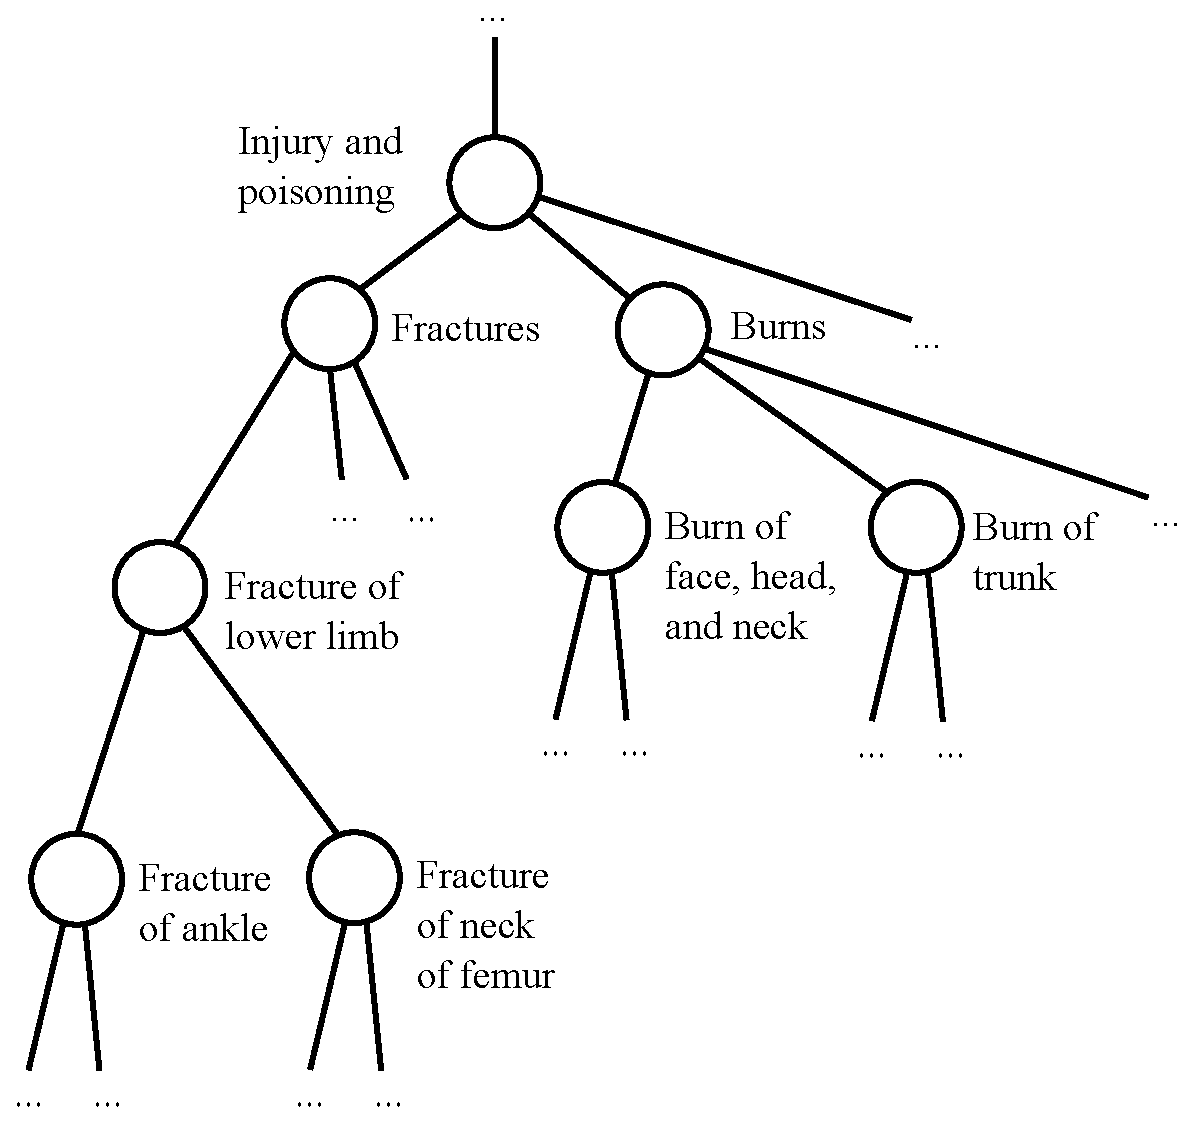
\includegraphics[scale=0.4]{Chapters/chapter1/figures/hi_quality_ICD9_tree_cropped} \caption{An illustration of a portion of the ICD9 hierarchy.}
\label{fig:diagnosis_tree}
\end{figure}


An automated process would ideally produce a more complete and accurate
diagnosis lists. %Also, this model will reveal information about the
%medical records themselves. For example, we may gain an understanding
%of what a specific code actually means in terms of clinical narratives.
The task of automatic ICD-9 coding has been investigated in the clinical
domain.  Methods used to solve this problem (besides HSLDA) range from applying manually derived coding rules
rules to applications of online rule learning approaches \cite{Crammer2007,Goldstein2007,Farkas2008}.
Many classification schemes have been applied to this problem: K-nearest
neighbor , Naive Bayes, support vector machines, Bayesian Ridge Regression, as
well as simple keyword mappings, all with promising
results~\cite{LarkeyCroft95,RibeiroNeto2001,PakhomovEtAl06,Lita2008}.%Ruch2008 omitted

%Much of the work was triggered by the 2007 medical NLP community
%challenge~\cite{Challenge07}.
%The data in the challenge, however, differs from 
%ours in its scope. The datasets were smaller (1,000 training and 1,000 testing
%documents) and focused on radiology reports with a restricted number of ICD-9
%codes (45 of them, compared to 7K+ in our dataset). 

The specific dataset we report results for in this chapter was gathered from the NewYork-Presbyterian Hospital clinical data warehouse. 
It consists of 6,000 discharge summaries and
their associated ICD-9 codes (7,298 distinct codes overall), representing a portion of
the discharges from the hospital in 2009. All included discharge summaries had associated ICD-9 Codes.
Summaries have 8.39 associated ICD-9
codes on average (std dev=5.01) and contain an average of 536.57 terms after
preprocessing (std dev=300.29). We split our dataset into 5,000 discharge
summaries for training and 1,000 for testing.

The text of the discharge summaries was tokenized with
NLTK.\footnote{http://www.nltk.org} A fixed vocabulary was formed by taking
the top 10,000 tokens with highest document frequency (exclusive of names,
places and other identifying numbers). The study was approved
by the Institutional Review Board and follows HIPAA (Health
Insurance Portability and Accountability Act) privacy guidelines.

Here HSLDA is evaluated as a way to understand and model the relationship between a discharge summary and the ICD-9 codes that should be assigned to it.  We show promising results for automatically assigning ICD-9 codes to hospital discharge records.  

%For each hospitalization there are usually several ICD-9 codes assigned
%for billing purposes. These codes are known to be quite specific but
%not very sensitive \cite{}. Regardless of that fact,
%this is one of the only sources for information on patient diagnoses
%aside from the free text. %Aside from prediction, one of the goals is to compare the sensitivity of predictions from the HSLDA model in comparison to the codes in a case where a test closer to ground truth is available. For this we will compare whether predictions for the ICD-9 code associated with anemia are better predicted by HSLDA or by the ICD-9 codes. Anemia was chosen because hemoglobin values are readily available and the definition of anemia according the World Health Organization is approximately 12.5, with a threshold of 12 for women and 13 for men [citation].

\subsection{Product Descriptions and Catalogs}

Many web-retailers store and organize their catalog of products in a
mulitply-rooted hierarchy in addition to providing textual product descriptions 
for most products. Products can be discovered by users
through free-text search and product category exploration. Top-level
product categories are displayed on the front page of the website and lower
level categories can be discovered by choosing one of the top-level categories.
Products can exist in multiple locations in the hierarchy.


\begin{figure}[t]
%tbp] %  figure placement: here, top, bottom, or page
\centering 
\includegraphics[scale=0.4]{Chapters/chapter1/figures/hi_quality_product_tree_cropped} \caption{An illustration of a portion of the Amazon product hierarchy.}
\label{fig:product_tree}
\end{figure}


Amazon.com is one such retailer.  Their product categorization data is available as part of the 
 Stanford Network Analysis Platform (SNAP) dataset~\cite{SNAP}.    A representative sub-tree of the amazon.com DVD product category tree is shown in Figure \ref{fig:product_tree}.  
Product descriptions were obtained separately from the
Amazon.com website directly. Once such description is
\begin{quote}
{Winner of five Academy Awards, including Best Picture and Best Director, The Deer Hunter 
is simultaneously an audacious directorial conceit and one of the greatest films ever made 
about friendship and the personal impact of war. Like Apocalypse Now, it's hardly a conventional 
battle film--the soldier's experience was handled with greater authenticity in Platoon--but its 
depiction of war on an intimate scale packs a devastatingly dramatic punch ... }
\end{quote}
We study the collection of DVDs
in the product catalog specifically.
%We were able to deduce the structure of the
%hierarchy for the Amazon.com products because all ancestors in the
%hierarchy were included with each category label. For example, {}``DVD / Genres
%/ Science Fiction \& Fantasy / Classic Sci-Fi'' is a single product category 
%for the DVD, {}``The Time Machine.''
The resulting dataset contains 15,130 product descriptions for training and 1,000
for testing. The product descriptions consist of
91.89 terms on average (std dev=53.08). Overall, there are 2,691 unique categories.
Products are assigned on average 9.01 categories (std dev=4.91). The vocabulary
consists of the most frequent 30,000 words omitting stopwords. 

HSLDA is used here to understand and model the relationship between the product text description and the products' positioning in the product hierarchy.  We show how to automatically situate a product in a hierarchal product catalog.  


\subsection{Comparison Models}

We compare HSLDA to two closely related models. The comparison models are SLDA with independent
regressors (hierarchical constraints on labels ignored,  i.e. the regression is not conditional) and HSLDA fit by first
performing LDA then fitting probit regressors that respect the conditional label hierarchy (rather than jointly inferring the topics and the regression coefficients). These models were
chosen because they are the strongest available competitors and because they  highlight several pedagogical aspects of HSLDA including performance in the
absence  of hierarchical constraints, the effect of the combined inference, and
regression performance attributable solely to the hierarchical constraints.

SLDA with independent regressors is the most salient comparison model
for our work. The distinguishing factor between HSLDA and SLDA is the
additional structure imposed on the label space, a distinction that in developing HDSLA we
hypothesized would result in a difference in predictive performance. 

 The second comparison model, HSLDA fit by performing LDA first
followed by performing inference over the hierarchically constrained label
space, does not allow
the responses to influence the topics inferred by LDA.
Combined inference has been shown to improve performance in SLDA
\cite{BleiMcAuliffe2008}. This comparison model does not examine the value of utilizing the structured nature 
of the label space, instead it highlights the benefit of combined inference over both the
documents and the label space. 

%The last comparison model is HSLDA with fixed and randomly selected regression
%parameters. There is a baseline benefit that the structure in the label space 
%provides for the prediction of labels. This comparison model is intended to
%quantify the contribution of the structure alone.

For all three models, particular attention was given to the settings of the 
prior parameters for the regression coefficients. These parameters implement an
important form of regularization in HSLDA. In the setting where there are no
negative labels, a Gaussian prior over the regression parameters with a
negative mean implements a prior belief that missing labels are likely to be
negative. Thus, we show model performance for all three models with a
range of values for $\mu$, the mean prior parameter for regression coefficients 
($\mu\in\left\{ -3,-2.8,-2.6,\ldots,1\right\}$).

The number of topics for all models was set to $K=50$, the prior distributions of
$p\left(\alpha\right)$, $p\left(\alpha^{\prime}\right)$, and
$p\left(\gamma\right)$ were all chosen to be gamma with a shape parameter of 1 and a
scale parameter of 1000.   Different values of $K$ corresponding to different numbers of topics were explored, however, the results that we show in the following are not substantially changed in character.  As is usual in mixed-membership models, there is an ideal number of topics that should be used for out-of-sample prediction tasks, however, a full model-selection search varying topic cardinality was not performed for these datasets.

\begin{figure}[h]
\begin{center}
%\subfloat[][\label{fig:1a}]{\includegraphics[width=.49\textwidth]{figs/amazon_pred_varying_mu}}
\subfigure[Clinical data performance.]{\label{fig:1a}\includegraphics[width=.48\textwidth]{Chapters/chapter1/figs/clin_pred_varying_mu}}
%\subfloat[][\label{fig:1c}]{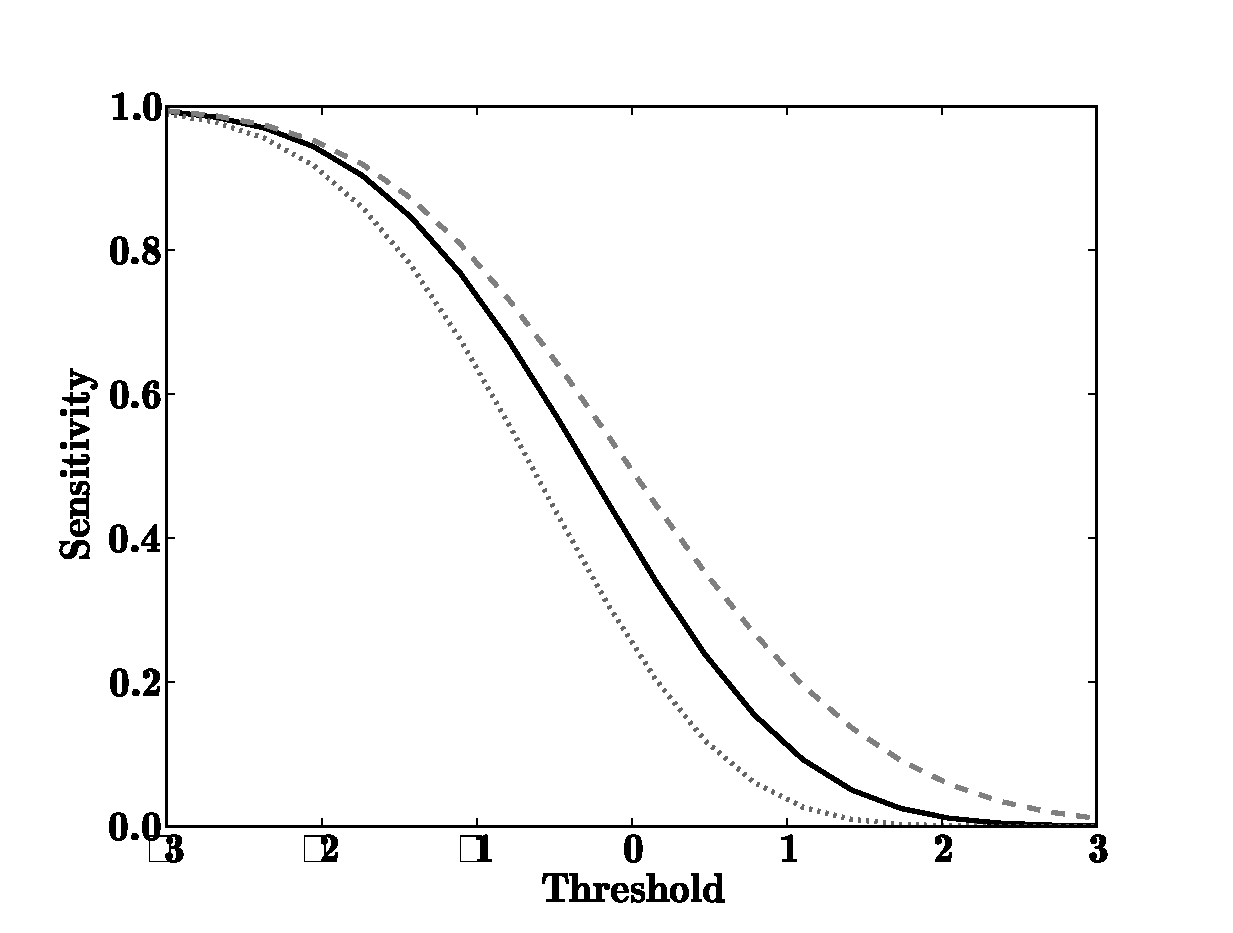
\includegraphics[width=.49\textwidth]{figs/sens_comparison_leafs}}
\subfigure[Retail product performance.]{\label{fig:1b}\includegraphics[width=.48\textwidth]{Chapters/chapter1/figs/amazon_pred_varying_mu}}
%\subfigure[][]{\label{fig:clinical_roc}\includegraphics[scale=0.4]{figs/ROC_comparison_leafs}}
\caption{ROC curves for HSLDA out-of-sample label prediction varying $\mu$, the prior mean of the regression parameters. 
In both figures, solid is HSLDA, dashed are independent regressors + SLDA (hierarchical 
constraints on labels ignored), and dotted is HSLDA fit by running LDA first then running 
tree-conditional regressions.}
%\label{fig:main_results}
\end{center}
\end{figure}


\subsection{Evaluation and Results}

%Outline:
%1. Model evaluation goal, metrics
%2. Gold standard(s), properties
%3. Method for prediction w/ details
%4. Discussion of results
%5. Connection of results with contribution and generality etc

We are particularly interested in
predictive performance on held-out data. Prediction performance was measured
with standard metrics -- sensitivity (true positive rate) and 1-specificity
(false positive rate). 

In each case the gold standard for testing was derived from the test data. To make the comparison as antagonistic to HSLDA as possible (relative to the other models), in evaluation only, ancestors of
observed nodes in the label hierarchy were ignored, observed nodes were
considered positive and descendants of observed nodes were assumed to be
negative. Note that this is different from our treatment of the observations during inference where we marginalize over possible settings of unobserved labels.
For instance, as the SLDA model does not enforce hierarchical
label constraints, when we consider only observed nodes we penalize HSLDA.  This is because
 the is-a hierarchical constraints say that the ancestors of positively labeled nodes must also be positive which the SLDA model cannot guarantee.
Another antagonism of this gold standard is that it is likely to inflate the number of false positives because
the labels applied to any particular document are usually not as complete as
they could be.  ICD-9 codes, for instance, are known to lack sensitivity and their use as a
gold standard could lead to correctly positive predictions being labeled as
false positives~\cite{Birmetal2005}.
However, given that the label space is often large (as in our examples) it is a
reasonable assumption that erroneous false positives should not skew results
significantly. 

Predictive performance in HSLDA is evaluated by computing
 \[p\left(y_{l,\hat{d}}\mid w_{1:N_{\hat{d}},\hat{d}}, w_{1:N_d,1:D},  y_{l\in\mathcal{L},1:D}\right)\] 
for each test document $\hat{d}$ for each observed label $y_{l,\hat{d}}$ (given the test document words). For efficiency, the expectation of this
probability distribution was approximated in the following way. Expectations 
of $\mathbf{\bar{z}}_{\hat{d}}$ and $\boldsymbol{\eta}_l$ were estimated with samples
from the posterior. Fixing these expectations, we performed Gibbs sampling over
the hierarchy to acquire predictive samples for the documents in the test set.
The true positive rate was calculated as the average expected labeling for
gold standard positive labels. The false positive rate was calculated 
as the average expected labeling for gold standard negative labels.

As sensitivity and specificity can always be traded off, we examined
sensitivity for a range of values for two different parameters -- the prior
means for the regression coefficients and the threshold for the auxiliary
variables.  The goal in this analysis was to evaluate the performance of these
models subject to more or less stringent requirements for predicting positive
labels. These two parameters have important related functions in the model. The
prior mean in combination with the auxiliary variable threshold together encode
the strength of the prior belief that unobserved labels are likely to be
negative. Effectively, the prior mean applies negative pressure to the
predictions and the auxiliary variable threshold determines the cutoff. 
For each model type, separate models were fit for each value of the 
prior mean of the regression coefficients.  This is a proper Bayesian
sensitivity analysis. In contrast, to evaluate
predictive performance as a function of the auxiliary variable threshold,
a single model was fit for each model type and prediction was evaluated
based on predictive samples drawn subject to different auxiliary variable
thresholds. These methods are significantly different since the prior mean
is varied prior to inference, and the auxiliary variable threshold is varied
following inference.
%However, as intended, they both highlight model performance 
%under more or less stringent requirements for predicting positive labels.

\begin{figure}[t]
%tbp] %  figure placement: here, top, bottom, or page
\centering \includegraphics[scale=0.4]{Chapters/chapter1/figs/ROC_comparison_leafs} \caption{ROC curve for out-of-sample ICD-9 code prediction varying auxiliary variable threshold. $\mu = -1.0$ for all three models in this figure.}
\label{fig:results_auxiliary_var} 
\end{figure}


Figure~\ref{fig:1a} demonstrates the performance of the model on the clinical data as an ROC curve varying $\mu$.  For instance, 
a hyperparameter setting of $\mu=-1.6$ yields the following performance:
the full HSLDA model had a 
true positive rate of 0.57 and a false positive rate of 0.13, the SLDA model
had a true positive rate of 0.42 and a false positive rate of 0.07, and the
HSLDA model where LDA and the regressions were fit separately had a true
positive rate of 0.39 and a false positive rate of 0.08. These points are highlighted in Figure~\ref{fig:1a}.  Note that the figure is somewhat misleading because for any one value of $\mu$ HSLDA outperforms the comparison models by a relatively large margin. 

These results indicate that the full HSLDA model predicts more of the the
correct labels at a cost of an increase in the number of false positives
relative to the comparison models.  However, as shown in Figure~\ref{fig:1a}  HSLDA outperforms or no worse than the comparison models across across the full range of specificities.  


Example topics (as word lists) learned for the discharge data are given below.  These word lists are computed by sorting
terms in decreasing order based on their probability under a given topic.

\begin{extract}
\begin{tabular}{|c|c|}
\hline
\textbf{Topic 1} & \textbf{Topic 2} \\ \hline \hline
MASS & WOUND \\
\hline
CANCER & FOOT \\
\hline
RIGHT & CELLULITIS \\
\hline
BREAST & ULCER \\
\hline
CHEMOTHERAPY & LEFT \\
\hline
METASTATIC & ERYTHEMA \\
\hline
LEFT & PAIN \\
\hline
LYMPH & SWELLING \\
\hline
TUMOR & SKIN \\
\hline
BIOPSY & RIGHT \\
\hline
CARCINOMA & ABSCESS \\
\hline
LUNG & LEG \\
\hline
CHEMO & OSTEOMYELITIS \\
\hline
ADENOCARCINOMA & TOE \\
\hline
NODE & DRAINAGE \\
\hline
\end{tabular}
\end{extract}

These topics closely correspond to common clinical concepts, namely, cancers of the thorax and wounds common to diabetics suffering from poor peripheral circulation.  Evaluations of the subject coherence of these topics relative to baselines are ongoing, but early results suggest positive findings similar to those reported for other supervised LDA models.

Figure~\ref{fig:1b} demonstrates the performance of the model on the retail product data as an ROC curve also varying $\mu$. For
instance, a hyperparameter setting of $\mu=-2.2$ yields the following
performance: the full HSLDA model had a true positive rate of 0.85 
and a false positive rate of 0.30, the SLDA model had a true positive
rate of 0.78 and a false positive rate of 0.14, and the HSLDA model where
LDA and the regressions were fit separately had a true positive rate of 0.77
and a false positive rate of 0.16. These results follow a similar pattern to the clinical data. These points are highlighted in Figure~\ref{fig:1b}.

Example topics (as word lists) learned for the amazon.com data are given below.  These word lists were also computed by sorting
terms in decreasing order based on their probability under a given topic.

\begin{extract}
\begin{tabular}{|c|c|}
\hline
\textbf{Topic 1} & \textbf{Topic 2} \\ \hline \hline
SERIES & BASEBALL \\
\hline
EPISODES & TEAM \\
\hline
SHOW & GAME \\
\hline
SEASON & PLAYERS \\
\hline
EPISODE & BASKETBALL \\
\hline
FIRST & SPORT \\
\hline
TELEVISION & SPORTS \\
\hline
SET & NEW \\
\hline
TIME & PLAYER \\
\hline
TWO & SEASON \\
\hline
SECOND & LEAGUE \\
\hline
ONE & FOOTBALL \\
\hline
CHARACTERS & STARS \\
\hline
DISC & FANS \\
\hline
GUEST & FIELD \\
\hline
\end{tabular}
\end{extract}

Figure \ref{fig:results_auxiliary_var} shows the predictive performance of HSLDA 
relative to the two comparison models on the clinical dataset as a function of the auxiliary variable threshold. 
For low values of the auxiliary variable threshold, the models predict labels
in a more sensitive and less specific manner, creating the points in the upper
right corner of the ROC curve. As the auxiliary variable threshold is
increased, the models predict in a less sensitive and more specific manner,
creating the points in the lower left hand corner of the ROC curve. HSLDA with full joint inference outperforms SLDA with
independent regressors as well as HSLDA with separately trained
regression. 

%\begin{figure}[t]
%%tbp] %  figure placement: here, top, bottom, or page
% \centering \includegraphics[scale=0.4]{figs/ROC_comparison_leafs} \caption{ROC curve for Out-of-sample ICD-9 code predictions.}
%\label{fig:clinical_roc} 
%\end{figure}

%Despite the proliferation of LDA related models in recent years, one could argue that the true killer app for LDA has yet to be discovered.  LDA makes sense for information retrieval (IR) because  the learned latent topic vectors serve as good low-dimensional document representations, and, a posteriori similarity between such vectors can be used to compute the similarity of documents.  Unfortunately, computational considerations render this approach to IR impractical in most settings.

The SLDA model family, of which HSLDA is a member, can be understood in two different ways.  One way is to see it as a family of topic models that improve on the topic modeling performance of LDA via the inclusion of observed supervision.  Another way to see the family is as a set of models that can predict labels for bag-of-words data.  A large diversity of problems can be expressed as label prediction problems for bag-of-words data.  A surprisingly large amount of that kind of data possess structured labels, either hierarchically constrained or otherwise.  That HSLDA directly addresses this kind of data is a large part of the motivation for this work.   That it outperforms more straightforward approaches should be of interest to practitioners.

Variational Bayes has been the predominant estimation approach applied to sLDA models.  Hierarchical probit regression makes for tractable Markov chain Monte Carlo SLDA inference, a benefit that should extend to other sLDA models should probit regression be used for response variable prediction there too.  

The results in Figures~\ref{fig:1a} and \ref{fig:1b} suggest that in most cases it is better to do full joint estimation of HSLDA.  In alternative interpretation of the same results is that if one is more sensitive to the performance gains that result from exploiting the structure of the labels then one can, in an engineering sense, get nearly as much gain in label prediction performance by first fitting LDA and then fitting a hierarchical probit regression.  There are applied settings in which this could be advantageous.

Extensions to this work include unbounded topic cardinality variants and relaxations to different kinds of label structure.  Unbounded topic cardinality variants pose interesting inference challenges.  Utilizing different kinds of label structure is possible within this framework, but requires relaxing some of the simplifications we made in this paper for expositional purposes. 

%We have described a mixed membership model with hierarchical supervision. We have demonstrated this model in the context of document modeling with hierarchical multi-label supervision. Such a model is appropriate in domains where there are hierarchical constraints among the labels such as is the case in an IS-A hierarchy.

...

%\begin{itemize}
%\item what about the nonparametric version of this?
%\item discuss the broader goal, from the beginning of search engine time, to combine categorization and free text.  this, to our knowledge, is the first principled approach to doing so
%\end{itemize}


\section{Appendix}
%\subsection{MCMC}
%\label{sec:mcmc}
%Markov chain Monte Carlo (MCMC) is the name given to a particular technique for generating samples from distributions of interest.  In Bayesian analyses this distribution is often the posterior distribution of the latent quantities given the data and fixed parameters.  The technique is general, elegant, and simple.  The basic idea is that by using Markov chain transition kernel templates, it is possible to construct and simulate a Markov chain whose equilibrium distribution is the distribution of interest.   This means that  the sequence of Markov chain simulation outputs can be used as an empirical stand-in approximation to the distribution of interest.  What is more, general MCMC techniques don't rely upon having a normalized probability distribution as a starting point, merely a function that is at all points proportional to the distribution of interest.   This is particularly convenient in the Bayesian case where the posterior distribution is of interest and does not have an analytic form.  In this case, the posterior distribution is simply proportion to the joint distribution with the observed quantities fixed to their observed values.

Let $\mathbf{z}$ be a set of latent variables.  Let $\mathbf{x}$ be a set of observed quantities.  We could denote by $\theta$ any set of fixed parameters and include it on the conditioning side of every expression to follow in this section but, since it would appear in every expression we'll omit it for purposes of notational clarity.  Our goal is to generate samples distributed according to $P(\mathbf{z} | \mathbf{x})$ (one can think about sampling from a posterior distribution here, however, MCMC applies more generally).  We have a model whose joint distribution is specified and can be evaluated readily for all settings of $\mathbf{z}$ and $\mathbf{x}$.  By Bayes rule we know that

\[P(\mathbf{z} | \mathbf{x} = (x_1, \ldots, x_N) ) \propto P(\mathbf{z}, \mathbf{x}= (x_1, \ldots, x_N)).\]

We denote by $\tilde{P}(\mathbf{z} | \mathbf{x} = (x_1, \ldots, x_N) )$ the normalized version of $P(\mathbf{z} | \mathbf{x} = (x_1, \ldots, x_N) )$.  Assume that we can come up with a function $P(\mathbf{z}^* | \mathbf{z})$ that has the following property (called )

\[P(\mathbf{z*} | \mathbf{x} = (x_1, \ldots, x_N) ) = \sum_ \mathbf{z} P(\mathbf{z}^* | \mathbf{z}) P(\mathbf{z} | \mathbf{x} = (x_1, \ldots, x_N) )\]
%\subsection{Auxiliary Variables}
\subsection{Probit Regression}
\label{sec:probit_review}

%\begin{figure}[htbp]
%\begin{center}
%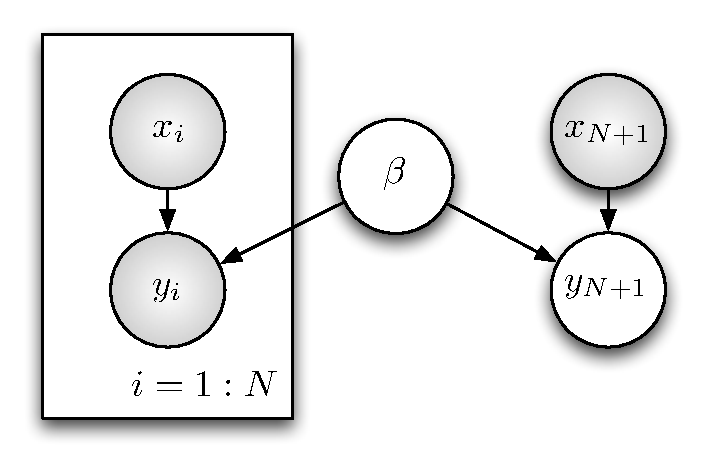
\includegraphics{Chapters/chapter1/probit_no_aux_vars}
%\caption{Probit model, no auxiliary variables}
%\label{fig:probit_no_aux_vars}
%\end{center}
%\end{figure}
%
%%
%%\begin{figure}[htbp]
%%\begin{center}
%%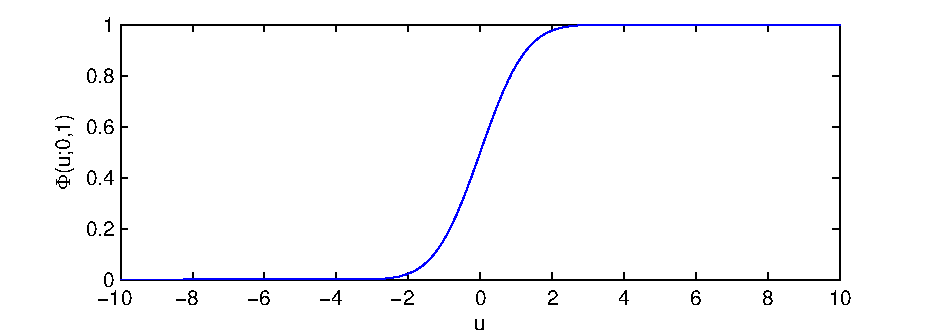
\includegraphics{Chapters/chapter1/cdf}
%%\caption{CDF of $N(0,1)$}
%%\label{fig:cdf}
%%\end{center}
%%\end{figure}
%
%\begin{figure}[htbp]
%\begin{center}
%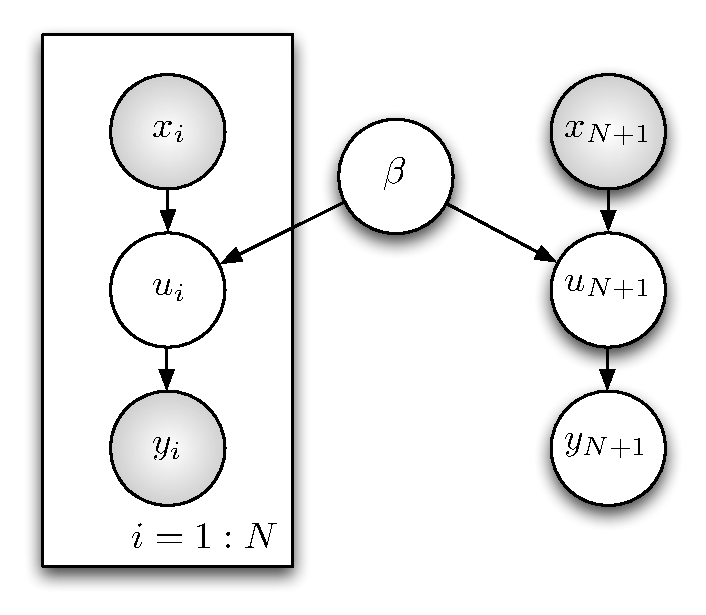
\includegraphics{Chapters/chapter1/probit}
%\caption{Probit model}
%\label{fig:probit}
%\end{center}
%\end{figure}




%For reasons that are somewhat obscure to me, statisticians tend to use probit regression for binary classification whereas machine learners tend to use logistic regression.  In a recent paper, my collaborators and I found it useful for computational purposes to use probit regression.  One can find many good primers on probit regression around the web, but, as we all know, there is almost always space for another.  
%
%Figure \ref{fig:cdf} is the cumulative distribution function (cdf) of a $N(0,1)$ distribution. 
%
For reasons that are somewhat obscure, statisticians tend to use probit regression for binary classification whereas machine learners tend to use logistic regression.
 The ``probit'' function is the inverse of the normal cumulative distribution function (cdf).    We denote the normal {\em cdf} function $\Phi(x;\mu,\sigma^2)$ with $\mu$ the mean, $\sigma^2$ the variance and $x$ the argument.

The range of the normal cdf is $(0,1)$ which means that it can be interpreted as a probability.  For instance, one can construct a generalized linear classification model (a ``probit regression model'') of the form 
\begin{equation}
P(y_i = 1) = \Phi(x_i^T\beta; 0, \sigma^2). \label{eqn:probit}
\end{equation}  Depending on convention (i.e. binary $y_i$ represented as $\{1,0\}$ or $\{1,-1\}$) then the probability of $y_i$ being labeled the opposite way is $P(y_i = -1)$ or $P(y_i = 0) = 1 - P(y_i=1).$  Here $x_i$ is a vector of covariates, $\beta$ is a vector of weights, and $y_i$ is a single, binary valued response.  The close relationship between regression and classification are in full display here : probit regression is a ``generalized linear {\em regression} model'' as well as a ``binary classifier.''

%Figure \ref{fig:probit_no_aux_vars} shows the graphical model for probit regression (minus any priors on the regression weights $\beta$).   
 In this model we would like to use labeled training data, $\{x_i, y_i\}_{i=1}^N$ to ``learn'' the value of $\beta$ and then to use this value to predict the value of $y_{N+1} | x_{N+1}, \beta.$  Being Bayesian about inference means that we will average over the posterior distribution of $\beta$ when making predictions.  This means that we want to draw samples from the posterior distribution of $\beta | \{x_i, y_i\}_{i=1}^N$.  To to this efficiently one can introduce a set of auxiliary variables $\{u_i\}_{i=1}^N$.  
 %In this note we will demonstrate that the model in  Figure \ref{fig:probit} is the same as the model in Figure \ref{fig:probit_no_aux_vars}  when the $u_i$'s are marginalized out and will suggest that inference in the former is computationally easier.  

By auxiliary variable we mean that such variables will be used as an intermediary for purposes of efficiency but will otherwise be uninteresting.    They are variables introduced into a model in order to make inference easier but whose existence does not change the distribution of interest.  Auxiliary variables for slice sampling are one particularly clever use of auxiliary variables.  The auxiliary variable trick in probit regression is another.

For the purposes of exposition, forget about the $i$ index for a bit and focus on a single instance $y$, $x$, and $u$.  The argument we make will hold for all by simply reintroducing subscripts.  

To start, let's propose a factorized joint distribution for these quantities

\begin{equation}
P(y,x,u) = P(y|u)P(u|x,\beta) \label{eqn:joint}
\end{equation}

Straight away, one can see why this auxiliary variable scheme works.  By the law of total probability we have
\begin{equation}
P(y,x) = \int P(y,x,u)du= \int P(y|u)P(u|x,\beta)du.  \label{eqn:joint_marginalized}
\end{equation}
So, if by some means we generate $S$ samples $\{u^{(s)},y^{(s)},x^{(s)}\}_{s=1}^S \sim P(y,x,u)$ we know that marginalizing $u$ out (i.e.~disregarding its value) we get samples $\{y^{(s)},x^{(s)}\}_{s=1}^S \sim P(y,x).$  %Equation  \ref{eqn:joint_marginalized} 
%\begin{eqnarray}
%y_i &\sim& \Phi(x_i^T\beta; 0, 1)
%\end{eqnarray}

We haven't specified the most important part of the auxiliary variable sampling scheme yet, namely, what $P(y|u)$ and what $P(u|x,\beta)$ are.   Let's try $y = \mbox{sign}(u)$ and $u \sim N(x^T\beta,\sigma^2).$  These choices are nice in a particular way.  First let's verify that the marginalization of $u$ out of this model results in the model specification in Equation \ref{eqn:probit}.

\begin{eqnarray*}
P(y=1|x,\beta) &=&  \int P(y=1|u)P(u|x,\beta)du\\
&=& \int \mathbb{I}(u>0)N(u;x^T\beta,\sigma^2) du \\
&=& \int_0^\infty N(u;x^T\beta,\sigma^2) du \\
&=& 1 - \Phi(0; x^T\beta,\sigma^2) \\ 
&=& \Phi(x^T\beta; 0, \sigma^2)
\end{eqnarray*}
where the last line comes from the fact that for symmetric distributions like the normal distribution, 
$\Phi(x^T\beta; 0, \sigma^2) = 1 - \Phi(-x^T\beta; 0, \sigma^2)$ and the mean of a normal cdf can be translated arbitrarily, i.e. $\Phi(-x^T\beta; 0, \sigma^2) = \Phi(0;x^T\beta, \sigma^2)$ (which comes from adding the offset $x^T\beta$ to the cdf argument and mean).  

Having established the fact that for a particular sort of auxiliary variable choice, we get the same probit model as we wanted, why is this choice nice?

Well, it comes down to sampling $\beta$ and $u$ and $y$.  Generally, sampling $\beta$ in the model without auxiliary variables will require hybrid Monte Carlo (HMC) or Metropolis Hastings of some sort.  Gibbs sampling often comes with substantial benefits.  By making this choice of auxiliary variable the conditional distribution of $u_i$ given everything else is proportional to a truncated Normal distribution, a distribution that is, by nature of its commonness, relatively straightforward to sample from.  The big benefit, though, acrues from the posterior form for sampling $\beta$.  With the $u$'s ``observed'' (as they would be in a Gibbs sampler), the posterior distribution of $\beta$ (for typical choices of prior) is precisely the same as that for linear regression, perhaps the most well studied model in statistics.  In that case, sampling $\beta$ from its posterior distribution is quite simple usually; certainly more so that sampling $\beta$ without the $u$ auxiliary variables.

The extension to the multivariate HSLDA setting is straightforward and follows this line of reasoning precisely.  An extended discussion of the techniques suggested here and the multivariate generalization can be found in \cite{gelmanbda04}.




%\begin{VF}
%``A Process is a structured, measured set of activities designed to produce a specific output for a particular customer
%or market---A process is thus a specific ordering of work activities across time and space, with a beginning, an end.
%and clearly defined inputs and outputs: a structure for action.''
%
%\VA{Thomas Davenport}{Senior Adjutant to the Junior Marketing VP}
%\end{VF}
%
%
%\begin{shadebox}
%A component part for an electronic item is
%manufactured at one of three different factories, and then delivered to
%the main assembly line.Of the total number supplied, factory A supplies
%50\%, factory B 30\%, and factory C 20\%. Of the components
%manufactured at factory A, 1\% are faulty and the corresponding
%proportions for factories B and C are 4\% and 2\% respectively. A
%component is picked at random from the assembly line. What is the
%probability that it is faulty? 
%\end{shadebox}
%
%In most literature on PPDP, they \cite{jolliffe2002pca} consider a more relaxed, yet more practical, notion of privacy protection by assuming limited attacker's background knowledge. Below, the term ``victim" refers to the record owner being linked. We can broadly classify linking models to two families.
%
%\begin{extract}
%A component part for an electronic item is \cite{hyvarinen2001ica}
%manufactured at one of three different factories, and then delivered to
%the main assembly line.Of the total number supplied, factory A supplies
%50\%, factory B 30\%, and factory C 20\%. Of the components
%manufactured at factory A, 1\% are faulty and the corresponding
%proportions for factories B and C are 4\% and 2\% respectively. 
%\end{extract}
%
%\begin{shortbox}
%\Boxhead{Box Title Here}
%Another family aims at achieving the \emph{uninformative principle}: The published table should provide the attacker with little additional information beyond the background knowledge. There should not be a large difference between the prior and posterior beliefs; otherwise, there is a privacy threat~\cite{jain2004ass, jolliffe2002pca}. Many privacy models in this family are designed for statistical database and do not distinguish attributes in $T$ into $QID$, but some of them could also thwart record, attribute, and table linkages. Section~\ref{intro} studies this family of privacy models.
%
%Let $m$ be a prime number. With the addition and multiplication as 
%defined above, $Z_m$ is a field.
%\end{shortbox}
%
%\begin{theorem}\label{1th:Z_m}
%Let $m$ be a prime number. With the addition and multiplication as 
%defined above, $Z_m$ is a field.
%\end{theorem}
%
%\begin{proof}
%Most of the proof of this theorem is routine.  It is clear that $0\in Z_m$ 
%and $1\in Z_m$ are the 
%zero element and identity element. If $a\in Z_m$ and $a\ne 0$, then $m-a$ 
%is the additive inverse of $a$. If $a\in Z_m$ and $a\ne 0$, then the 
%greatest common divisor of $a$ and $m$ is 1, and hence
%there exist integers $s$ and $t$ such that $sa+tm=1$. Thus $sa=1 -tm$ is 
%congruent to 1 modulo $m$. Let $s^*$ be the integer in $Z_m$ 
%congruent to $s$ 
%modulo $m$. Then we also have $s^*a\equiv 1\  \mbox{mod}\ m$. Hence $s^*$ 
%is 
%the multiplicative inverse of $a$ modulo $m$. Verification of the rest of 
%the field properties is now routine.\end{proof}
%
%\begin{definition}\label{1def:linearcomb}{\rm
%Let $u^{(1)},u^{(2)},\ldots,u^{(m)}$ be vectors in $F^n$, and let 
%$c_1,c_2,\ldots,c_m$ be scalars. Then the vector
%\[c_1u^{(1)}+c_2u^{(2)}+\cdots+c_mu^{(m)}\]
%is called a {\it linear combination} \index{linear combination} of $u^{(1)},u^{(2)},\ldots,u^{(m)}$.
%If $V$ is a subspace of $F^n$, then $V$ is closed under vector addition and 
%scalar multiplication, and it follows easily by induction that a 
%linear combination of vectors in $V$ is also a vector in $V$. Thus 
%{\it subspaces 
%are closed under linear combinations}; in fact, this can be taken as the 
%defining property of subspaces.
%The vectors $u^{(1)},u^{(2)},\ldots,u^{(m)}$ {\it span} $V$ \index{spanning set}
%(equivalently, form a {\it spanning set} of $V$) provided every vector in 
%$V$ 
%is a linear combination of $u^{(1)},u^{(2)},\ldots,u^{(m)}$. The zero 
%vector can be written as a linear combination of 
%$u^{(1)},u^{(2)},\ldots,u^{(m)}$ with all scalars equal to 0; this is a 
%{\it trivial linear combination}.\index{linear combination!trivial} The vectors
%$u^{(1)},u^{(2)},\ldots,u^{(m)}$ are {\it linearly dependent} provided 
%there are scalars $c_1,c_2,\ldots,c_m$, not all of which are zero, such 
%that
%\[c_1u^{(1)}+c_2u^{(2)}+\cdots+c_mu^{(m)}=0,\]
%that is, the zero vector can be written as a {\it nontrivial linear \index{linear combination!nontrivial} 
%combination} of $u^{(1)},u^{(2)},\ldots,u^{(m)}$.
%For example, the vectors $(1,4), (3,-1)$, and $(3,5)$ in $\Re^2$ are 
%linearly 
%dependent since
%\[3(1,4)+1(3,-2)-2(3,5)=(0,0).\] Vectors are {\it linearly independent} provided  they are not linearly dependent.\index{linearly independent}
%The vectors 
%$u^{(1)},u^{(2)},\ldots,u^{(m)}$ are a {\it basis} \index{basis} of $V$ provided they are  
%linearly independent and span $V$.
%By an {\it ordered basis} \index{basis!ordered} we mean a basis in which the vectors of the basis are listed 
%in a specified order; to indicate that we have an ordered basis we write
%$(u^{(1)},u^{(2)},\ldots,u^{(m)})$. 
%A spanning set $S$ of $V$ is a \index{spanning set!minimal} {\it minimal spanning set of $V$} provided that
%each set 
%of vectors obtained from $S$ by removing a vector is not a spanning set 
%for $V$.
%A linearly independent set $S$ of vectors of $V$ is a {\it maximal linearly \index{linearly independent!maximal}
%independent set of vectors of $V$} provided that for each vector $w$ of 
%$V$ that 
%is not in $S$, $S\cup\{w\}$ is  linearly dependent (when this happens, 
%$w$ must be  a linear combination of the vectors in 
%$S$).\hfill{$\Box$}
%}\end{definition}
%
%In addition to matrix addition, subtraction, and multiplication, there is 
%one additional operation that we define now. It's perhaps the simplest of 
%them all. Let $A=[a_{ij}]$ be an $m$ by $n$ matrix and let $c$ be a 
%number \cite{hyvarinen2001ica}. Then the matrix $c\cdot A$, or simply $cA$, is the $m$ by $n$ 
%matrix obtained by multiplying each entry of $A$ by $c$:
%\[c A=[ca_{ij}].\]\index{matrix!scalar multiplication} \index{matrix!scalar multiple of}
%The matrix $c A$ is called a {\it scalar multiple} of $A$.
%
%\begin{VT1}
%
%\VH{Think About It...}
%
%Commonly thought of as the first modern computer, ENTAC was built in 1944. It took up more space than an 18-wheeler's
%tractor trailer and weighed more than 17 Chevrolet Camaros. It consumed 140,000 watts of electricity while executing
%up to 5,000 basic arithmetic operations per second. One of today's popular microprocessors, the 486, is built on a
%tiny piece of silicon about the size of a dime.
%
%\VT
%With the continual expansion of capabilities, computing power will eventually exceed the capacity for human
%comprehension or human control.
%
%\VTA{The Information Revolution}{Business Week}
%\end{VT1}
%
%
%\section{Glossary}
%\begin{Glossary}
%\item[360 Degree Review] Performance review that includes feedback from superiors, peers, subordinates, and clients.
%\item[Abnormal Variation] Changes in process performance that cannot be accounted for by typical day-to-day variation. Also referred to as
%non-random variation.
%\item[Acceptable Quality Level (AQL)] The minimum number of parts that must comply with quality standards, usually stated as a percentage.
%\item[Activity] The tasks performed to change inputs into outputs.
%\item[Adaptable] An adaptable process is designed to maintain effectiveness and efficiency as requirements change. The process is
%deemed adaptable when there is agreement among suppliers, owners, and customers that the process will meet
%requirements throughout the strategic period.
%\end{Glossary}
%


